\documentclass[twoside]{book}

% Packages required by doxygen
\usepackage{fixltx2e}
\usepackage{calc}
\usepackage{doxygen}
\usepackage[export]{adjustbox} % also loads graphicx
\usepackage{graphicx}
\usepackage[utf8]{inputenc}
\usepackage{makeidx}
\usepackage{multicol}
\usepackage{multirow}
\PassOptionsToPackage{warn}{textcomp}
\usepackage{textcomp}
\usepackage[nointegrals]{wasysym}
\usepackage[table]{xcolor}

% Font selection
\usepackage[T1]{fontenc}
\usepackage[scaled=.90]{helvet}
\usepackage{courier}
\usepackage{amssymb}
\usepackage{sectsty}
\renewcommand{\familydefault}{\sfdefault}
\allsectionsfont{%
  \fontseries{bc}\selectfont%
  \color{darkgray}%
}
\renewcommand{\DoxyLabelFont}{%
  \fontseries{bc}\selectfont%
  \color{darkgray}%
}
\newcommand{\+}{\discretionary{\mbox{\scriptsize$\hookleftarrow$}}{}{}}

% Page & text layout
\usepackage{geometry}
\geometry{%
  a4paper,%
  top=2.5cm,%
  bottom=2.5cm,%
  left=2.5cm,%
  right=2.5cm%
}
\tolerance=750
\hfuzz=15pt
\hbadness=750
\setlength{\emergencystretch}{15pt}
\setlength{\parindent}{0cm}
\setlength{\parskip}{3ex plus 2ex minus 2ex}
\makeatletter
\renewcommand{\paragraph}{%
  \@startsection{paragraph}{4}{0ex}{-1.0ex}{1.0ex}{%
    \normalfont\normalsize\bfseries\SS@parafont%
  }%
}
\renewcommand{\subparagraph}{%
  \@startsection{subparagraph}{5}{0ex}{-1.0ex}{1.0ex}{%
    \normalfont\normalsize\bfseries\SS@subparafont%
  }%
}
\makeatother

% Headers & footers
\usepackage{fancyhdr}
\pagestyle{fancyplain}
\fancyhead[LE]{\fancyplain{}{\bfseries\thepage}}
\fancyhead[CE]{\fancyplain{}{}}
\fancyhead[RE]{\fancyplain{}{\bfseries\leftmark}}
\fancyhead[LO]{\fancyplain{}{\bfseries\rightmark}}
\fancyhead[CO]{\fancyplain{}{}}
\fancyhead[RO]{\fancyplain{}{\bfseries\thepage}}
\fancyfoot[LE]{\fancyplain{}{}}
\fancyfoot[CE]{\fancyplain{}{}}
\fancyfoot[RE]{\fancyplain{}{\bfseries\scriptsize Generated by Doxygen }}
\fancyfoot[LO]{\fancyplain{}{\bfseries\scriptsize Generated by Doxygen }}
\fancyfoot[CO]{\fancyplain{}{}}
\fancyfoot[RO]{\fancyplain{}{}}
\renewcommand{\footrulewidth}{0.4pt}
\renewcommand{\chaptermark}[1]{%
  \markboth{#1}{}%
}
\renewcommand{\sectionmark}[1]{%
  \markright{\thesection\ #1}%
}

% Indices & bibliography
\usepackage{natbib}
\usepackage[titles]{tocloft}
\setcounter{tocdepth}{3}
\setcounter{secnumdepth}{5}
\makeindex

% Hyperlinks (required, but should be loaded last)
\usepackage{ifpdf}
\ifpdf
  \usepackage[pdftex,pagebackref=true]{hyperref}
\else
  \usepackage[ps2pdf,pagebackref=true]{hyperref}
\fi
\hypersetup{%
  colorlinks=true,%
  linkcolor=blue,%
  citecolor=blue,%
  unicode%
}

% Custom commands
\newcommand{\clearemptydoublepage}{%
  \newpage{\pagestyle{empty}\cleardoublepage}%
}

\usepackage{caption}
\captionsetup{labelsep=space,justification=centering,font={bf},singlelinecheck=off,skip=4pt,position=top}

%===== C O N T E N T S =====

\begin{document}

% Titlepage & ToC
\hypersetup{pageanchor=false,
             bookmarksnumbered=true,
             pdfencoding=unicode
            }
\pagenumbering{alph}
\begin{titlepage}
\vspace*{7cm}
\begin{center}%
{\Large Project A\+D\+BO \\[1ex]\large 0.\+42b }\\
\vspace*{1cm}
{\large Generated by Doxygen 1.8.12}\\
\end{center}
\end{titlepage}
\clearemptydoublepage
\pagenumbering{roman}
\tableofcontents
\clearemptydoublepage
\pagenumbering{arabic}
\hypersetup{pageanchor=true}

%--- Begin generated contents ---
\chapter{Hierarchical Index}
\section{Class Hierarchy}
This inheritance list is sorted roughly, but not completely, alphabetically\+:\begin{DoxyCompactList}
\item \contentsline{section}{Can\+Move}{\pageref{interface_can_move}}{}
\begin{DoxyCompactList}
\item \contentsline{section}{Runner}{\pageref{class_runner}}{}
\end{DoxyCompactList}
\item \contentsline{section}{High\+Score\+Script}{\pageref{class_high_score_script}}{}
\item Mono\+Behaviour\begin{DoxyCompactList}
\item \contentsline{section}{Back\+Ground}{\pageref{class_back_ground}}{}
\item \contentsline{section}{Credit\+Controller}{\pageref{class_credit_controller}}{}
\item \contentsline{section}{Game\+Controller}{\pageref{class_game_controller}}{}
\item \contentsline{section}{Game\+Over}{\pageref{class_game_over}}{}
\item \contentsline{section}{Main\+Menu\+Controller}{\pageref{class_main_menu_controller}}{}
\item \contentsline{section}{Obstacle}{\pageref{class_obstacle}}{}
\begin{DoxyCompactList}
\item \contentsline{section}{Flying\+Obstacle}{\pageref{class_flying_obstacle}}{}
\item \contentsline{section}{On\+The\+Ground\+Obstacle}{\pageref{class_on_the_ground_obstacle}}{}
\end{DoxyCompactList}
\item \contentsline{section}{Preference\+Controller}{\pageref{class_preference_controller}}{}
\item \contentsline{section}{Quit\+Controller}{\pageref{class_quit_controller}}{}
\item \contentsline{section}{Runner}{\pageref{class_runner}}{}
\item \contentsline{section}{Siang\+Malam}{\pageref{class_siang_malam}}{}
\item \contentsline{section}{Sounds\+Controller}{\pageref{class_sounds_controller}}{}
\end{DoxyCompactList}
\end{DoxyCompactList}

\chapter{Class Index}
\section{Class List}
Here are the classes, structs, unions and interfaces with brief descriptions\+:\begin{DoxyCompactList}
\item\contentsline{section}{\hyperlink{class_back_ground}{Back\+Ground} \\*Kelas \hyperlink{class_back_ground}{Back\+Ground} mengatur background pada Game\+Scene. }{\pageref{class_back_ground}}{}
\item\contentsline{section}{\hyperlink{interface_can_move}{Can\+Move} }{\pageref{interface_can_move}}{}
\item\contentsline{section}{\hyperlink{class_credit_controller}{Credit\+Controller} \\*Kelas \hyperlink{class_credit_controller}{Credit\+Controller} mengontrol Credit\+Scene. }{\pageref{class_credit_controller}}{}
\item\contentsline{section}{\hyperlink{class_flying_obstacle}{Flying\+Obstacle} \\*Kelas \hyperlink{class_flying_obstacle}{Flying\+Obstacle} merepresentasikan obstacle yang dapat terbang. }{\pageref{class_flying_obstacle}}{}
\item\contentsline{section}{\hyperlink{class_game_controller}{Game\+Controller} \\*Kelas \hyperlink{class_game_controller}{Game\+Controller} mengatur score game. }{\pageref{class_game_controller}}{}
\item\contentsline{section}{\hyperlink{class_game_over}{Game\+Over} \\*Kelas \hyperlink{class_game_over}{Game\+Over} merepresentasikan game saat game over. }{\pageref{class_game_over}}{}
\item\contentsline{section}{\hyperlink{class_high_score_script}{High\+Score\+Script} }{\pageref{class_high_score_script}}{}
\item\contentsline{section}{\hyperlink{class_main_menu_controller}{Main\+Menu\+Controller} \\*Kelas \hyperlink{class_main_menu_controller}{Main\+Menu\+Controller} mengontrol Main\+Menu\+Scene. }{\pageref{class_main_menu_controller}}{}
\item\contentsline{section}{\hyperlink{class_obstacle}{Obstacle} \\*Kelas abstract \hyperlink{class_obstacle}{Obstacle} merepresentasikan obstacle. }{\pageref{class_obstacle}}{}
\item\contentsline{section}{\hyperlink{class_on_the_ground_obstacle}{On\+The\+Ground\+Obstacle} \\*Kelas \hyperlink{class_on_the_ground_obstacle}{On\+The\+Ground\+Obstacle} merepresentasikan obstacle yang berada di atas tanah. }{\pageref{class_on_the_ground_obstacle}}{}
\item\contentsline{section}{\hyperlink{class_preference_controller}{Preference\+Controller} \\*Kelas \hyperlink{class_preference_controller}{Preference\+Controller} mengontrol Preference\+Scene. }{\pageref{class_preference_controller}}{}
\item\contentsline{section}{\hyperlink{class_quit_controller}{Quit\+Controller} \\*Kelas \hyperlink{class_quit_controller}{Quit\+Controller} mengontrol Quit\+Scene. }{\pageref{class_quit_controller}}{}
\item\contentsline{section}{\hyperlink{class_runner}{Runner} \\*Kelas \hyperlink{class_runner}{Runner} merepresentasikan runner. }{\pageref{class_runner}}{}
\item\contentsline{section}{\hyperlink{class_siang_malam}{Siang\+Malam} \\*Kelas \hyperlink{class_siang_malam}{Siang\+Malam} mengatur siang malam di gamr. }{\pageref{class_siang_malam}}{}
\item\contentsline{section}{\hyperlink{class_sounds_controller}{Sounds\+Controller} \\*Kelas Sounds controller mengontrol suara pada game. }{\pageref{class_sounds_controller}}{}
\end{DoxyCompactList}

\chapter{File Index}
\section{File List}
Here is a list of all files with brief descriptions\+:\begin{DoxyCompactList}
\item\contentsline{section}{C\+:/\+Users/\+Public/\+Documents/\+Unity Projects/\+Ellena/\+Ta\+Daa/\+Megaman Endless Run/\+Assets/\+Controller/\+Script/\hyperlink{_credit_controller_8cs}{Credit\+Controller.\+cs} }{\pageref{_credit_controller_8cs}}{}
\item\contentsline{section}{C\+:/\+Users/\+Public/\+Documents/\+Unity Projects/\+Ellena/\+Ta\+Daa/\+Megaman Endless Run/\+Assets/\+Controller/\+Script/\hyperlink{_flying_obstacle_8cs}{Flying\+Obstacle.\+cs} }{\pageref{_flying_obstacle_8cs}}{}
\item\contentsline{section}{C\+:/\+Users/\+Public/\+Documents/\+Unity Projects/\+Ellena/\+Ta\+Daa/\+Megaman Endless Run/\+Assets/\+Controller/\+Script/\hyperlink{_game_over_8cs}{Game\+Over.\+cs} }{\pageref{_game_over_8cs}}{}
\item\contentsline{section}{C\+:/\+Users/\+Public/\+Documents/\+Unity Projects/\+Ellena/\+Ta\+Daa/\+Megaman Endless Run/\+Assets/\+Controller/\+Script/\hyperlink{_main_menu_controller_8cs}{Main\+Menu\+Controller.\+cs} }{\pageref{_main_menu_controller_8cs}}{}
\item\contentsline{section}{C\+:/\+Users/\+Public/\+Documents/\+Unity Projects/\+Ellena/\+Ta\+Daa/\+Megaman Endless Run/\+Assets/\+Controller/\+Script/\hyperlink{_obstacle_8cs}{Obstacle.\+cs} }{\pageref{_obstacle_8cs}}{}
\item\contentsline{section}{C\+:/\+Users/\+Public/\+Documents/\+Unity Projects/\+Ellena/\+Ta\+Daa/\+Megaman Endless Run/\+Assets/\+Controller/\+Script/\hyperlink{_on_the_ground_obstacle_8cs}{On\+The\+Ground\+Obstacle.\+cs} }{\pageref{_on_the_ground_obstacle_8cs}}{}
\item\contentsline{section}{C\+:/\+Users/\+Public/\+Documents/\+Unity Projects/\+Ellena/\+Ta\+Daa/\+Megaman Endless Run/\+Assets/\+Controller/\+Script/\hyperlink{_preference_controller_8cs}{Preference\+Controller.\+cs} }{\pageref{_preference_controller_8cs}}{}
\item\contentsline{section}{C\+:/\+Users/\+Public/\+Documents/\+Unity Projects/\+Ellena/\+Ta\+Daa/\+Megaman Endless Run/\+Assets/\+Controller/\+Script/\hyperlink{_quit_controller_8cs}{Quit\+Controller.\+cs} }{\pageref{_quit_controller_8cs}}{}
\item\contentsline{section}{C\+:/\+Users/\+Public/\+Documents/\+Unity Projects/\+Ellena/\+Ta\+Daa/\+Megaman Endless Run/\+Assets/\+Controller/\+Script/\hyperlink{_sounds_controller_8cs}{Sounds\+Controller.\+cs} }{\pageref{_sounds_controller_8cs}}{}
\item\contentsline{section}{C\+:/\+Users/\+Public/\+Documents/\+Unity Projects/\+Ellena/\+Ta\+Daa/\+Megaman Endless Run/\+Assets/\+Model/\+Script/\hyperlink{_can_move_8cs}{Can\+Move.\+cs} }{\pageref{_can_move_8cs}}{}
\item\contentsline{section}{C\+:/\+Users/\+Public/\+Documents/\+Unity Projects/\+Ellena/\+Ta\+Daa/\+Megaman Endless Run/\+Assets/\+Model/\+Script/\hyperlink{_high_score_8cs}{High\+Score.\+cs} }{\pageref{_high_score_8cs}}{}
\item\contentsline{section}{C\+:/\+Users/\+Public/\+Documents/\+Unity Projects/\+Ellena/\+Ta\+Daa/\+Megaman Endless Run/\+Assets/\+View/\+Script/\hyperlink{_back_ground_8cs}{Back\+Ground.\+cs} }{\pageref{_back_ground_8cs}}{}
\item\contentsline{section}{C\+:/\+Users/\+Public/\+Documents/\+Unity Projects/\+Ellena/\+Ta\+Daa/\+Megaman Endless Run/\+Assets/\+View/\+Script/\hyperlink{_game_controller_8cs}{Game\+Controller.\+cs} }{\pageref{_game_controller_8cs}}{}
\item\contentsline{section}{C\+:/\+Users/\+Public/\+Documents/\+Unity Projects/\+Ellena/\+Ta\+Daa/\+Megaman Endless Run/\+Assets/\+View/\+Script/\hyperlink{_runner_8cs}{Runner.\+cs} }{\pageref{_runner_8cs}}{}
\item\contentsline{section}{C\+:/\+Users/\+Public/\+Documents/\+Unity Projects/\+Ellena/\+Ta\+Daa/\+Megaman Endless Run/\+Assets/\+View/\+Script/\hyperlink{_siang_malam_8cs}{Siang\+Malam.\+cs} }{\pageref{_siang_malam_8cs}}{}
\end{DoxyCompactList}

\chapter{Class Documentation}
\hypertarget{class_back_ground}{}\section{Back\+Ground Class Reference}
\label{class_back_ground}\index{Back\+Ground@{Back\+Ground}}


Kelas \hyperlink{class_back_ground}{Back\+Ground} mengatur background pada Game\+Scene.  


Inheritance diagram for Back\+Ground\+:\begin{figure}[H]
\begin{center}
\leavevmode
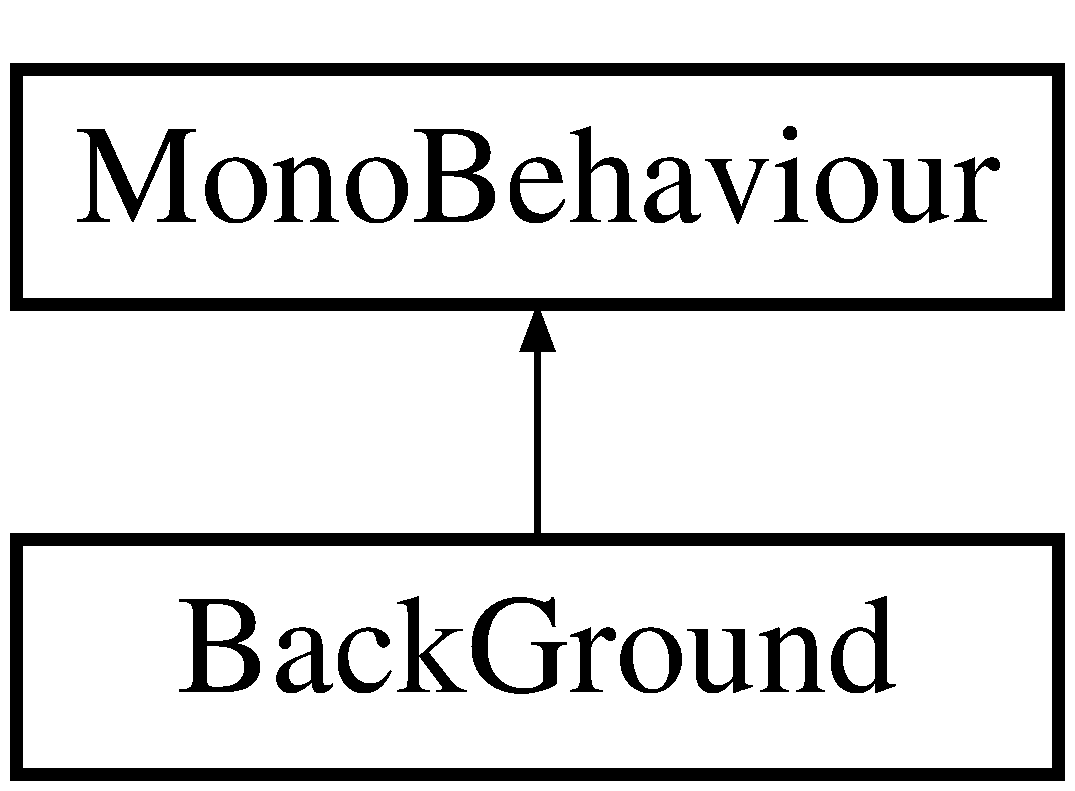
\includegraphics[height=2.000000cm]{class_back_ground}
\end{center}
\end{figure}


\subsection{Detailed Description}
Kelas \hyperlink{class_back_ground}{Back\+Ground} mengatur background pada Game\+Scene. 



The documentation for this class was generated from the following file\+:\begin{DoxyCompactItemize}
\item 
C\+:/\+Users/\+Public/\+Documents/\+Unity Projects/\+Ellena/\+Ta\+Daa/\+Megaman Endless Run/\+Assets/\+View/\+Script/\hyperlink{_back_ground_8cs}{Back\+Ground.\+cs}\end{DoxyCompactItemize}

\hypertarget{interface_can_move}{}\section{Can\+Move Interface Reference}
\label{interface_can_move}\index{Can\+Move@{Can\+Move}}
Inheritance diagram for Can\+Move\+:\begin{figure}[H]
\begin{center}
\leavevmode
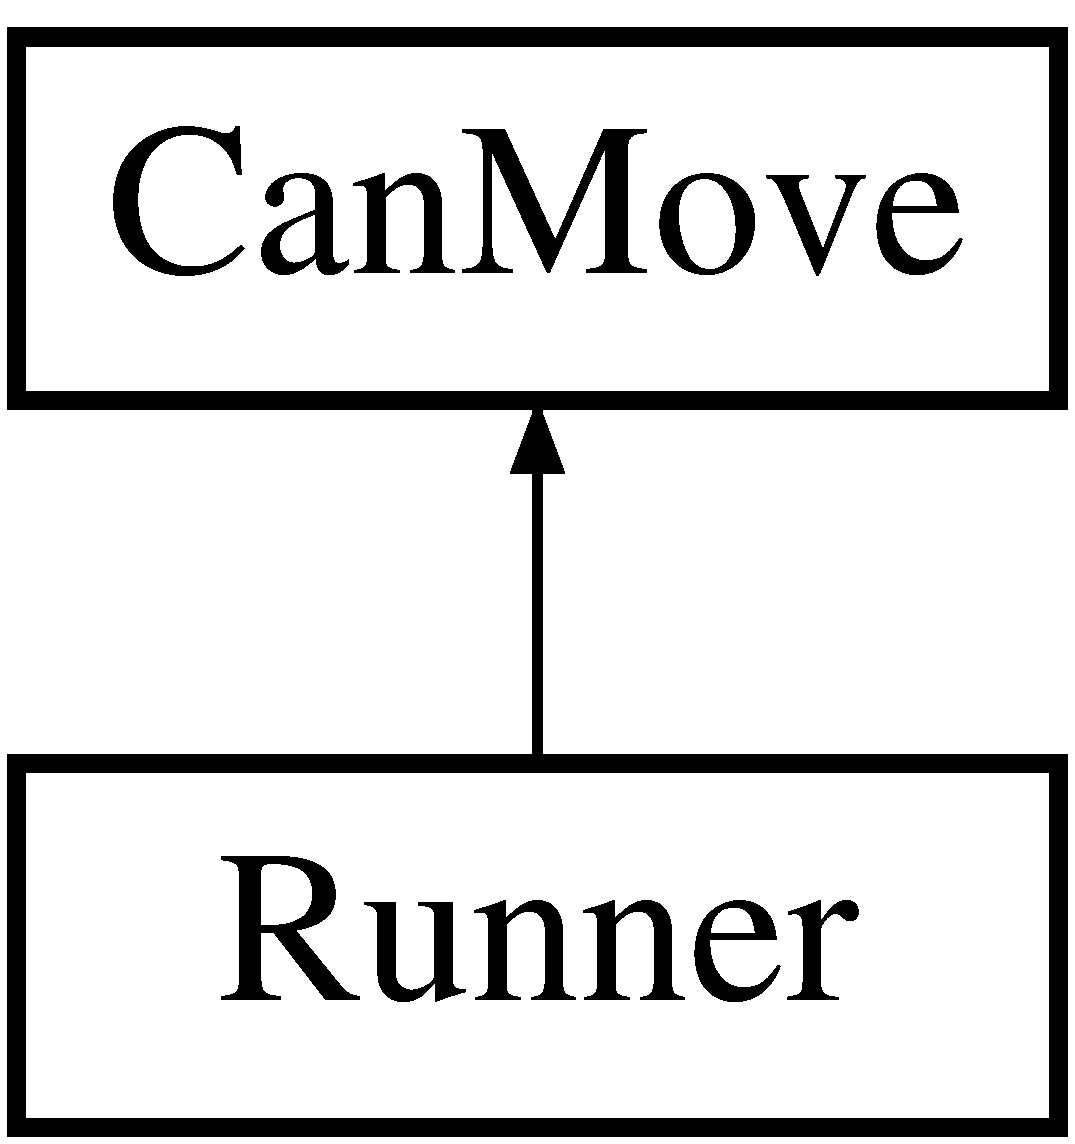
\includegraphics[height=2.000000cm]{interface_can_move}
\end{center}
\end{figure}
\subsection*{Public Member Functions}
\begin{DoxyCompactItemize}
\item 
void \hyperlink{interface_can_move_a2c40a4dc4684e8f04e31ff59d4ec74e0}{Move} ()
\end{DoxyCompactItemize}


\subsection{Member Function Documentation}
\hypertarget{interface_can_move_a2c40a4dc4684e8f04e31ff59d4ec74e0}{}\label{interface_can_move_a2c40a4dc4684e8f04e31ff59d4ec74e0} 
\index{Can\+Move@{Can\+Move}!Move@{Move}}
\index{Move@{Move}!Can\+Move@{Can\+Move}}
\subsubsection{\texorpdfstring{Move()}{Move()}}
{\footnotesize\ttfamily void Can\+Move.\+Move (\begin{DoxyParamCaption}{ }\end{DoxyParamCaption})}



Implemented in \hyperlink{class_runner_add0c89849fa2e023ed488ba80c7daf4a}{Runner}.



The documentation for this interface was generated from the following file\+:\begin{DoxyCompactItemize}
\item 
C\+:/\+Users/\+Public/\+Documents/\+Unity Projects/\+Ellena/\+Ta\+Daa/\+Megaman Endless Run/\+Assets/\+Model/\+Script/\hyperlink{_can_move_8cs}{Can\+Move.\+cs}\end{DoxyCompactItemize}

\hypertarget{class_credit_controller}{}\section{Credit\+Controller Class Reference}
\label{class_credit_controller}\index{Credit\+Controller@{Credit\+Controller}}


Kelas \hyperlink{class_credit_controller}{Credit\+Controller} mengontrol Credit\+Scene.  


Inheritance diagram for Credit\+Controller\+:\begin{figure}[H]
\begin{center}
\leavevmode
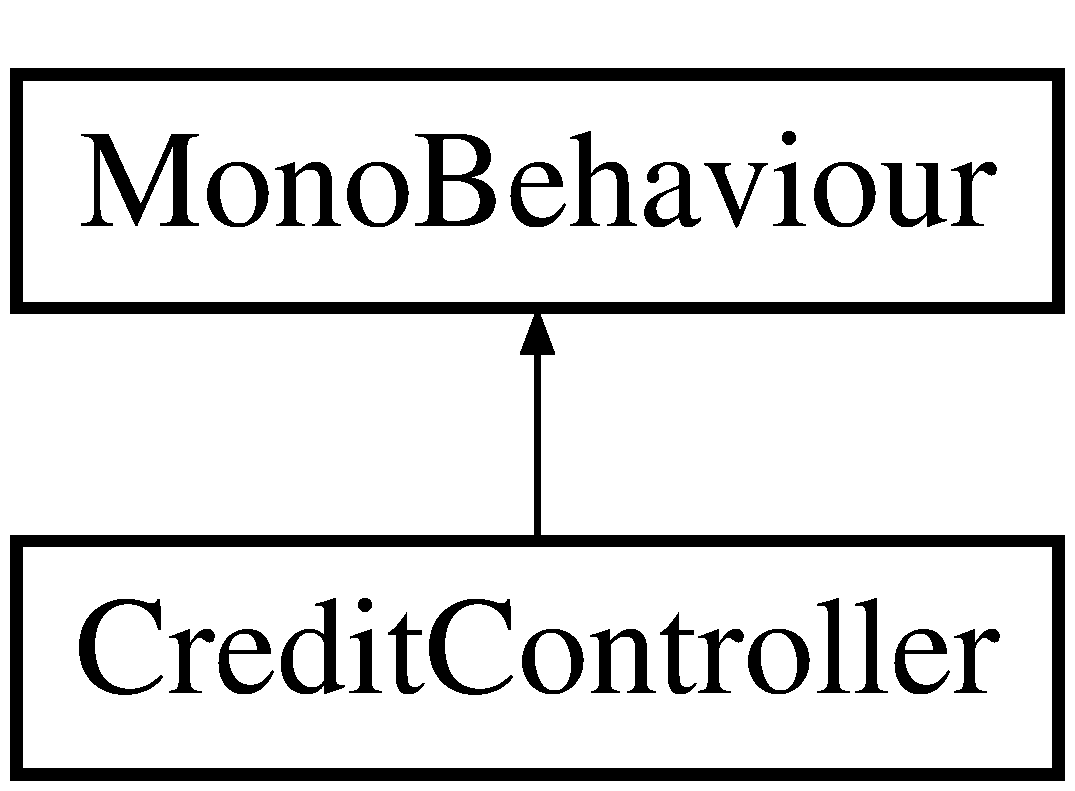
\includegraphics[height=2.000000cm]{class_credit_controller}
\end{center}
\end{figure}
\subsection*{Public Member Functions}
\begin{DoxyCompactItemize}
\item 
void \hyperlink{class_credit_controller_ad486d59710cfdbb207f0c4835143f86d}{main\+Menu\+Btn\+On\+Click} ()
\begin{DoxyCompactList}\small\item\em Mengatur tindakan yang dilakukan saat button Start\+Game\+Button diklik. Tindakan \+: Memulai game. \end{DoxyCompactList}\end{DoxyCompactItemize}
\subsection*{Public Attributes}
\begin{DoxyCompactItemize}
\item 
Button \hyperlink{class_credit_controller_a8b122365e9edd7291df09824506f726d}{Main\+Menu\+Button}
\begin{DoxyCompactList}\small\item\em Button -\/ button yang ada di Credit\+Scene. \end{DoxyCompactList}\end{DoxyCompactItemize}


\subsection{Detailed Description}
Kelas \hyperlink{class_credit_controller}{Credit\+Controller} mengontrol Credit\+Scene. 



\subsection{Member Function Documentation}
\hypertarget{class_credit_controller_ad486d59710cfdbb207f0c4835143f86d}{}\label{class_credit_controller_ad486d59710cfdbb207f0c4835143f86d} 
\index{Credit\+Controller@{Credit\+Controller}!main\+Menu\+Btn\+On\+Click@{main\+Menu\+Btn\+On\+Click}}
\index{main\+Menu\+Btn\+On\+Click@{main\+Menu\+Btn\+On\+Click}!Credit\+Controller@{Credit\+Controller}}
\subsubsection{\texorpdfstring{main\+Menu\+Btn\+On\+Click()}{mainMenuBtnOnClick()}}
{\footnotesize\ttfamily void Credit\+Controller.\+main\+Menu\+Btn\+On\+Click (\begin{DoxyParamCaption}{ }\end{DoxyParamCaption})}



Mengatur tindakan yang dilakukan saat button Start\+Game\+Button diklik. Tindakan \+: Memulai game. 



\subsection{Member Data Documentation}
\hypertarget{class_credit_controller_a8b122365e9edd7291df09824506f726d}{}\label{class_credit_controller_a8b122365e9edd7291df09824506f726d} 
\index{Credit\+Controller@{Credit\+Controller}!Main\+Menu\+Button@{Main\+Menu\+Button}}
\index{Main\+Menu\+Button@{Main\+Menu\+Button}!Credit\+Controller@{Credit\+Controller}}
\subsubsection{\texorpdfstring{Main\+Menu\+Button}{MainMenuButton}}
{\footnotesize\ttfamily Button Credit\+Controller.\+Main\+Menu\+Button}



Button -\/ button yang ada di Credit\+Scene. 



The documentation for this class was generated from the following file\+:\begin{DoxyCompactItemize}
\item 
C\+:/\+Users/\+Public/\+Documents/\+Unity Projects/\+Ellena/\+Ta\+Daa/\+Megaman Endless Run/\+Assets/\+Controller/\+Script/\hyperlink{_credit_controller_8cs}{Credit\+Controller.\+cs}\end{DoxyCompactItemize}

\hypertarget{class_flying_obstacle}{}\section{Flying\+Obstacle Class Reference}
\label{class_flying_obstacle}\index{Flying\+Obstacle@{Flying\+Obstacle}}


Kelas \hyperlink{class_flying_obstacle}{Flying\+Obstacle} merepresentasikan obstacle yang dapat terbang.  


Inheritance diagram for Flying\+Obstacle\+:\begin{figure}[H]
\begin{center}
\leavevmode
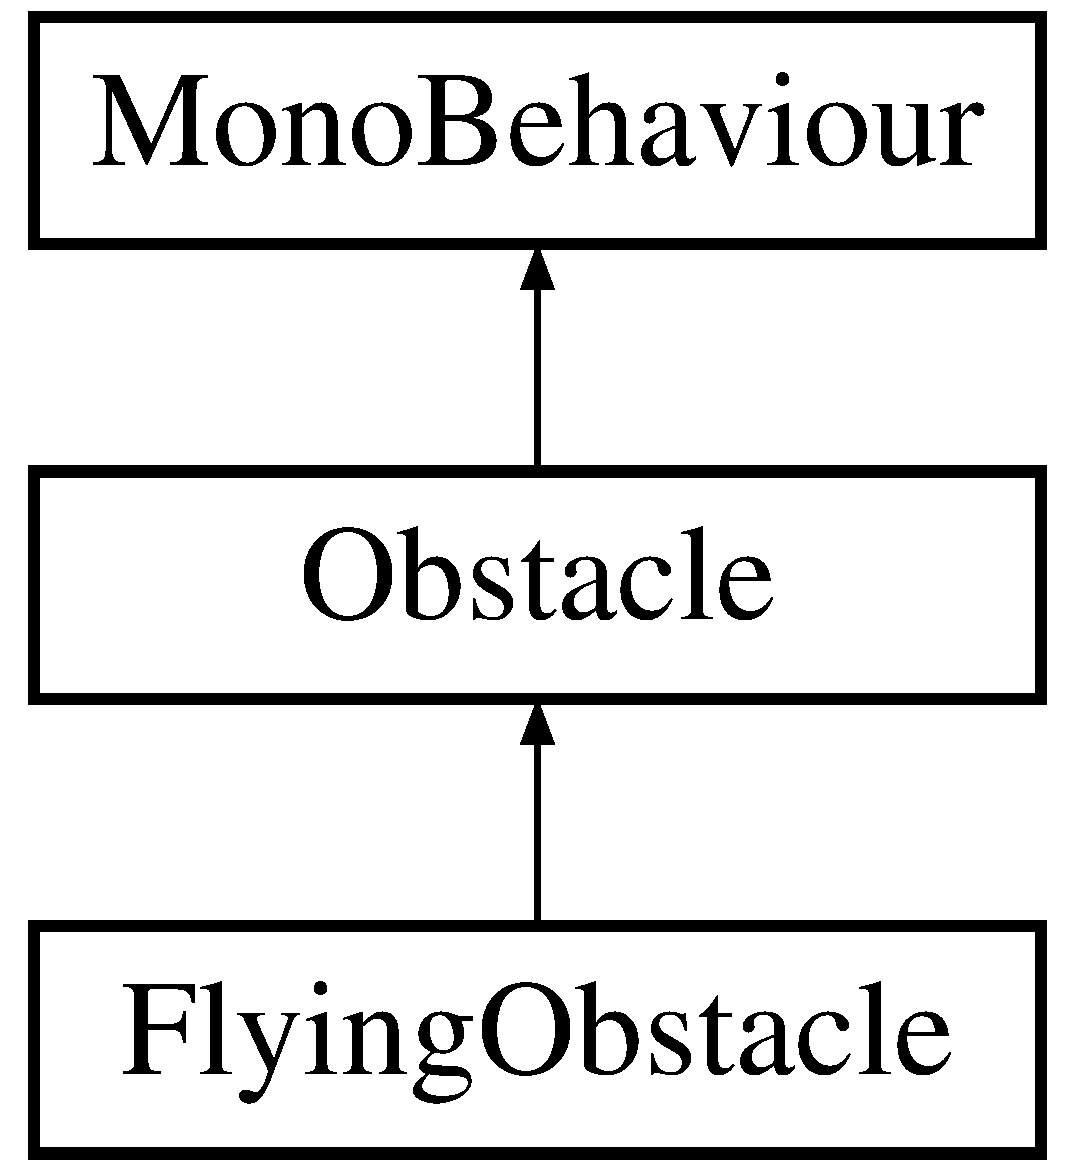
\includegraphics[height=3.000000cm]{class_flying_obstacle}
\end{center}
\end{figure}
\subsection*{Public Member Functions}
\begin{DoxyCompactItemize}
\item 
override void \hyperlink{class_flying_obstacle_a1c21c97ab8d9efa1c120103a2cd5cb34}{Obstacle\+Maker} ()
\begin{DoxyCompactList}\small\item\em Membuat \hyperlink{class_obstacle}{Obstacle}. \end{DoxyCompactList}\end{DoxyCompactItemize}
\subsection*{Additional Inherited Members}


\subsection{Detailed Description}
Kelas \hyperlink{class_flying_obstacle}{Flying\+Obstacle} merepresentasikan obstacle yang dapat terbang. 



\subsection{Member Function Documentation}
\hypertarget{class_flying_obstacle_a1c21c97ab8d9efa1c120103a2cd5cb34}{}\label{class_flying_obstacle_a1c21c97ab8d9efa1c120103a2cd5cb34} 
\index{Flying\+Obstacle@{Flying\+Obstacle}!Obstacle\+Maker@{Obstacle\+Maker}}
\index{Obstacle\+Maker@{Obstacle\+Maker}!Flying\+Obstacle@{Flying\+Obstacle}}
\subsubsection{\texorpdfstring{Obstacle\+Maker()}{ObstacleMaker()}}
{\footnotesize\ttfamily override void Flying\+Obstacle.\+Obstacle\+Maker (\begin{DoxyParamCaption}{ }\end{DoxyParamCaption})\hspace{0.3cm}{\ttfamily [virtual]}}



Membuat \hyperlink{class_obstacle}{Obstacle}. 



Implements \hyperlink{class_obstacle_a19f2f5d2c3176ee9ea8840862c55aa42}{Obstacle}.



The documentation for this class was generated from the following file\+:\begin{DoxyCompactItemize}
\item 
C\+:/\+Users/\+Public/\+Documents/\+Unity Projects/\+Ellena/\+Ta\+Daa/\+Megaman Endless Run/\+Assets/\+Controller/\+Script/\hyperlink{_flying_obstacle_8cs}{Flying\+Obstacle.\+cs}\end{DoxyCompactItemize}

\hypertarget{class_game_controller}{}\section{Game\+Controller Class Reference}
\label{class_game_controller}\index{Game\+Controller@{Game\+Controller}}


Kelas \hyperlink{class_game_controller}{Game\+Controller} mengatur score game.  


Inheritance diagram for Game\+Controller\+:\begin{figure}[H]
\begin{center}
\leavevmode
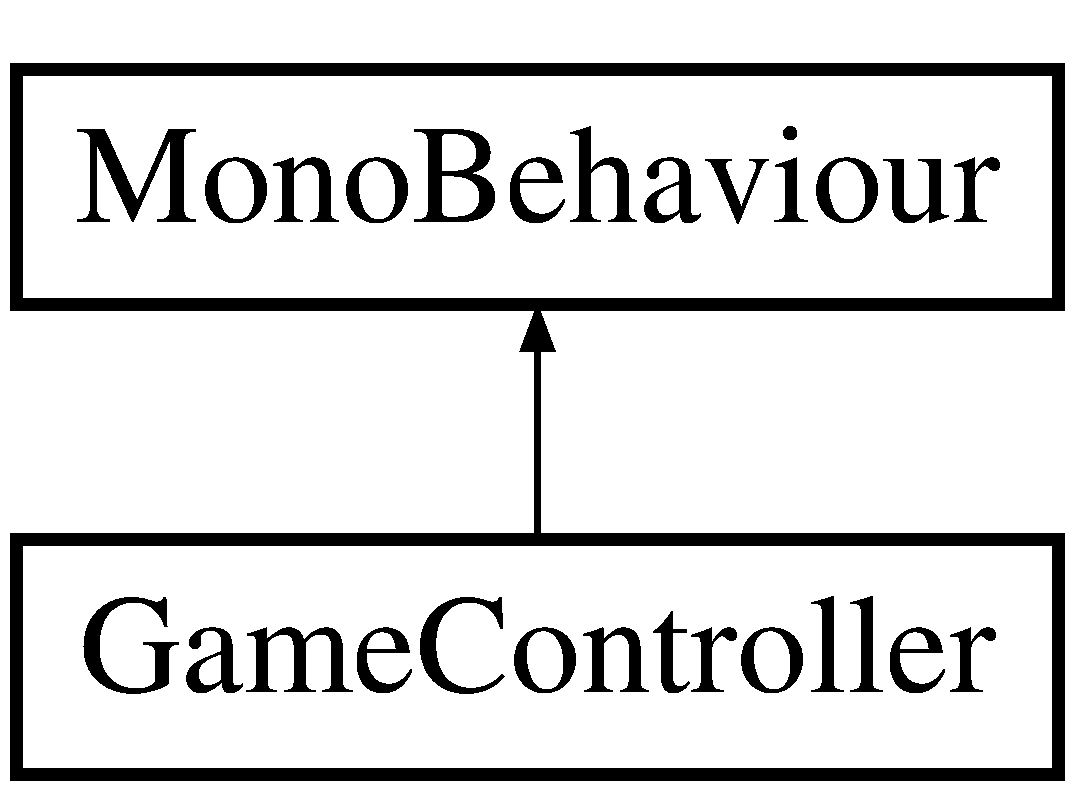
\includegraphics[height=2.000000cm]{class_game_controller}
\end{center}
\end{figure}
\subsection*{Public Attributes}
\begin{DoxyCompactItemize}
\item 
G\+U\+I\+Style \hyperlink{class_game_controller_a2aac028a07d314dc16cc7e78afef4ca6}{style1}
\begin{DoxyCompactList}\small\item\em Style G\+UI. \end{DoxyCompactList}\end{DoxyCompactItemize}


\subsection{Detailed Description}
Kelas \hyperlink{class_game_controller}{Game\+Controller} mengatur score game. 



\subsection{Member Data Documentation}
\hypertarget{class_game_controller_a2aac028a07d314dc16cc7e78afef4ca6}{}\label{class_game_controller_a2aac028a07d314dc16cc7e78afef4ca6} 
\index{Game\+Controller@{Game\+Controller}!style1@{style1}}
\index{style1@{style1}!Game\+Controller@{Game\+Controller}}
\subsubsection{\texorpdfstring{style1}{style1}}
{\footnotesize\ttfamily G\+U\+I\+Style Game\+Controller.\+style1}



Style G\+UI. 



The documentation for this class was generated from the following file\+:\begin{DoxyCompactItemize}
\item 
C\+:/\+Users/\+Public/\+Documents/\+Unity Projects/\+Ellena/\+Ta\+Daa/\+Megaman Endless Run/\+Assets/\+View/\+Script/\hyperlink{_game_controller_8cs}{Game\+Controller.\+cs}\end{DoxyCompactItemize}

\hypertarget{class_game_over}{}\section{Game\+Over Class Reference}
\label{class_game_over}\index{Game\+Over@{Game\+Over}}


Kelas \hyperlink{class_game_over}{Game\+Over} merepresentasikan game saat game over.  


Inheritance diagram for Game\+Over\+:\begin{figure}[H]
\begin{center}
\leavevmode
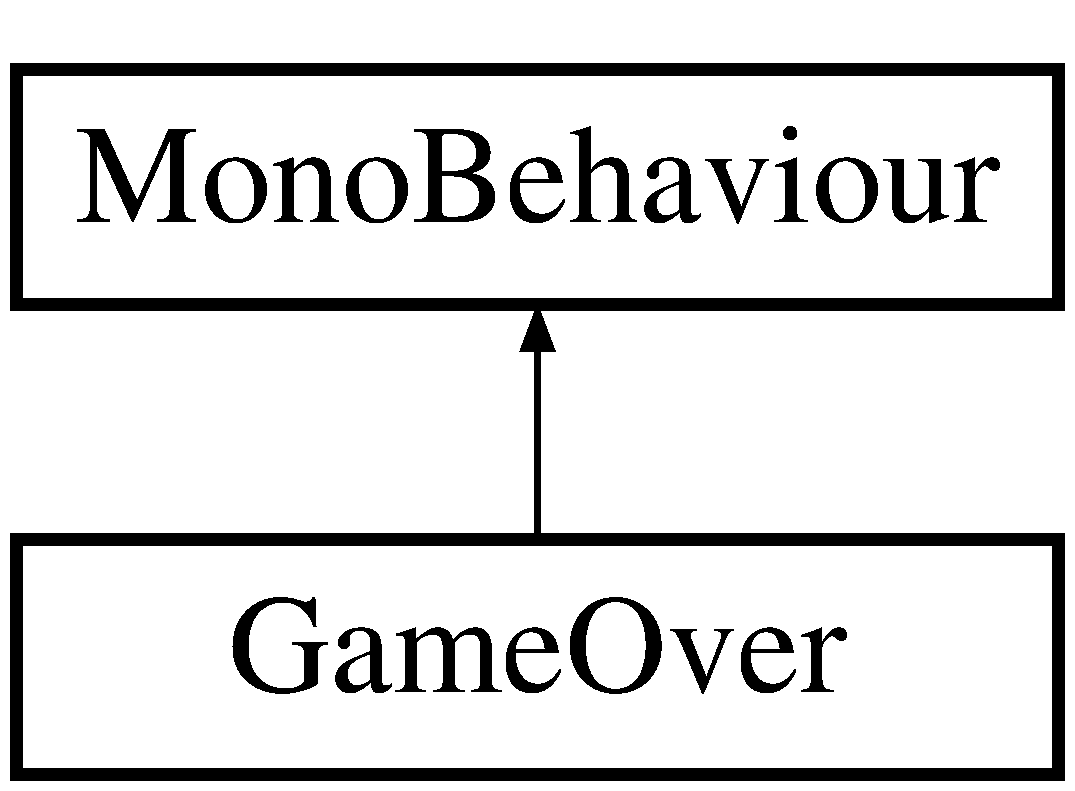
\includegraphics[height=2.000000cm]{class_game_over}
\end{center}
\end{figure}
\subsection*{Public Attributes}
\begin{DoxyCompactItemize}
\item 
G\+U\+I\+Style \hyperlink{class_game_over_a71e12fb4df1725763589943e10d7d9ec}{style2}
\begin{DoxyCompactList}\small\item\em Style G\+UI. \end{DoxyCompactList}\item 
Texture \hyperlink{class_game_over_ace41c3a08ba092a634f4b4b92c358e12}{retry}
\begin{DoxyCompactList}\small\item\em Texture Retry. \end{DoxyCompactList}\item 
Texture \hyperlink{class_game_over_aeffb99ea771f8eb04e5fe5c4c7dc71b2}{to\+Main\+Menu}
\begin{DoxyCompactList}\small\item\em Texture main menu. \end{DoxyCompactList}\item 
Camera \hyperlink{class_game_over_a899a798fa536c25b7c9781ee8c3ab9fd}{cam}
\end{DoxyCompactItemize}


\subsection{Detailed Description}
Kelas \hyperlink{class_game_over}{Game\+Over} merepresentasikan game saat game over. 



\subsection{Member Data Documentation}
\hypertarget{class_game_over_a899a798fa536c25b7c9781ee8c3ab9fd}{}\label{class_game_over_a899a798fa536c25b7c9781ee8c3ab9fd} 
\index{Game\+Over@{Game\+Over}!cam@{cam}}
\index{cam@{cam}!Game\+Over@{Game\+Over}}
\subsubsection{\texorpdfstring{cam}{cam}}
{\footnotesize\ttfamily Camera Game\+Over.\+cam}

\hypertarget{class_game_over_ace41c3a08ba092a634f4b4b92c358e12}{}\label{class_game_over_ace41c3a08ba092a634f4b4b92c358e12} 
\index{Game\+Over@{Game\+Over}!retry@{retry}}
\index{retry@{retry}!Game\+Over@{Game\+Over}}
\subsubsection{\texorpdfstring{retry}{retry}}
{\footnotesize\ttfamily Texture Game\+Over.\+retry}



Texture Retry. 

\hypertarget{class_game_over_a71e12fb4df1725763589943e10d7d9ec}{}\label{class_game_over_a71e12fb4df1725763589943e10d7d9ec} 
\index{Game\+Over@{Game\+Over}!style2@{style2}}
\index{style2@{style2}!Game\+Over@{Game\+Over}}
\subsubsection{\texorpdfstring{style2}{style2}}
{\footnotesize\ttfamily G\+U\+I\+Style Game\+Over.\+style2}



Style G\+UI. 

\hypertarget{class_game_over_aeffb99ea771f8eb04e5fe5c4c7dc71b2}{}\label{class_game_over_aeffb99ea771f8eb04e5fe5c4c7dc71b2} 
\index{Game\+Over@{Game\+Over}!to\+Main\+Menu@{to\+Main\+Menu}}
\index{to\+Main\+Menu@{to\+Main\+Menu}!Game\+Over@{Game\+Over}}
\subsubsection{\texorpdfstring{to\+Main\+Menu}{toMainMenu}}
{\footnotesize\ttfamily Texture Game\+Over.\+to\+Main\+Menu}



Texture main menu. 



The documentation for this class was generated from the following file\+:\begin{DoxyCompactItemize}
\item 
C\+:/\+Users/\+Public/\+Documents/\+Unity Projects/\+Ellena/\+Ta\+Daa/\+Megaman Endless Run/\+Assets/\+Controller/\+Script/\hyperlink{_game_over_8cs}{Game\+Over.\+cs}\end{DoxyCompactItemize}

\hypertarget{class_high_score_script}{}\section{High\+Score\+Script Class Reference}
\label{class_high_score_script}\index{High\+Score\+Script@{High\+Score\+Script}}
\subsection*{Static Public Attributes}
\begin{DoxyCompactItemize}
\item 
static int \hyperlink{class_high_score_script_a481a30c3e39d2e330f78346ac0424113}{high\+Scores} =0
\item 
static bool \hyperlink{class_high_score_script_a3f1b9e311b60157195b01e31b1e6b6d1}{game\+Over} = false
\end{DoxyCompactItemize}


\subsection{Member Data Documentation}
\hypertarget{class_high_score_script_a3f1b9e311b60157195b01e31b1e6b6d1}{}\label{class_high_score_script_a3f1b9e311b60157195b01e31b1e6b6d1} 
\index{High\+Score\+Script@{High\+Score\+Script}!game\+Over@{game\+Over}}
\index{game\+Over@{game\+Over}!High\+Score\+Script@{High\+Score\+Script}}
\subsubsection{\texorpdfstring{game\+Over}{gameOver}}
{\footnotesize\ttfamily bool High\+Score\+Script.\+game\+Over = false\hspace{0.3cm}{\ttfamily [static]}}

\hypertarget{class_high_score_script_a481a30c3e39d2e330f78346ac0424113}{}\label{class_high_score_script_a481a30c3e39d2e330f78346ac0424113} 
\index{High\+Score\+Script@{High\+Score\+Script}!high\+Scores@{high\+Scores}}
\index{high\+Scores@{high\+Scores}!High\+Score\+Script@{High\+Score\+Script}}
\subsubsection{\texorpdfstring{high\+Scores}{highScores}}
{\footnotesize\ttfamily int High\+Score\+Script.\+high\+Scores =0\hspace{0.3cm}{\ttfamily [static]}}



The documentation for this class was generated from the following file\+:\begin{DoxyCompactItemize}
\item 
C\+:/\+Users/\+Public/\+Documents/\+Unity Projects/\+Ellena/\+Ta\+Daa/\+Megaman Endless Run/\+Assets/\+Model/\+Script/\hyperlink{_high_score_8cs}{High\+Score.\+cs}\end{DoxyCompactItemize}

\hypertarget{class_main_menu_controller}{}\section{Main\+Menu\+Controller Class Reference}
\label{class_main_menu_controller}\index{Main\+Menu\+Controller@{Main\+Menu\+Controller}}


Kelas \hyperlink{class_main_menu_controller}{Main\+Menu\+Controller} mengontrol Main\+Menu\+Scene.  


Inheritance diagram for Main\+Menu\+Controller\+:\begin{figure}[H]
\begin{center}
\leavevmode
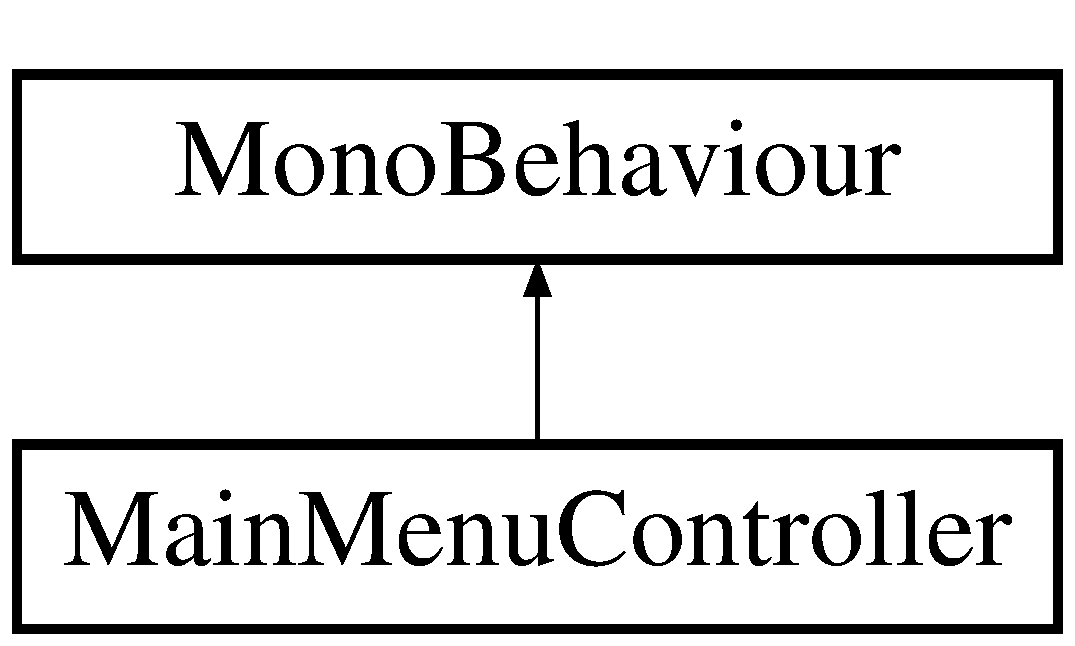
\includegraphics[height=2.000000cm]{class_main_menu_controller}
\end{center}
\end{figure}
\subsection*{Public Member Functions}
\begin{DoxyCompactItemize}
\item 
void \hyperlink{class_main_menu_controller_a3093b0f91bebcc757bd100be4ec19951}{start\+Game\+Btn\+On\+Click} ()
\begin{DoxyCompactList}\small\item\em Mengatur tindakan yang dilakukan saat button Start\+Game\+Button diklik. Tindakan \+: Memulai game. \end{DoxyCompactList}\item 
void \hyperlink{class_main_menu_controller_a4d4f79fdc5194e108997fb2b034bc144}{pref\+Btn\+On\+Click} ()
\begin{DoxyCompactList}\small\item\em Mengatur tindakan yang dilakukan saat button Preference\+Button diklik. Tindakan \+: Memunculkan layar Preference. \end{DoxyCompactList}\item 
void \hyperlink{class_main_menu_controller_a62a67c2d468bf4b4b45b1eefac4e08e0}{credit\+Btn\+On\+Click} ()
\begin{DoxyCompactList}\small\item\em Mengatur tindakan yang dilakukan saat button Credit\+Button diklik. Tindakan \+: Memunculkan layar Credit. \end{DoxyCompactList}\item 
void \hyperlink{class_main_menu_controller_a55f91b182c0d99e5697dd8a45aafb82b}{quit\+Btn\+On\+Click} ()
\begin{DoxyCompactList}\small\item\em Mengatur tindakan yang dilakukan saat button Quit\+Button diklik. Tindakan \+: Memunculkan layar Quit. \end{DoxyCompactList}\end{DoxyCompactItemize}
\subsection*{Public Attributes}
\begin{DoxyCompactItemize}
\item 
Button \hyperlink{class_main_menu_controller_ac8ee65de25015adeee8ee06dca4ff70a}{Start\+Game\+Button}
\begin{DoxyCompactList}\small\item\em Button -\/ button yang ada di Main\+Menu\+Scene. \end{DoxyCompactList}\end{DoxyCompactItemize}


\subsection{Detailed Description}
Kelas \hyperlink{class_main_menu_controller}{Main\+Menu\+Controller} mengontrol Main\+Menu\+Scene. 



\subsection{Member Function Documentation}
\hypertarget{class_main_menu_controller_a62a67c2d468bf4b4b45b1eefac4e08e0}{}\label{class_main_menu_controller_a62a67c2d468bf4b4b45b1eefac4e08e0} 
\index{Main\+Menu\+Controller@{Main\+Menu\+Controller}!credit\+Btn\+On\+Click@{credit\+Btn\+On\+Click}}
\index{credit\+Btn\+On\+Click@{credit\+Btn\+On\+Click}!Main\+Menu\+Controller@{Main\+Menu\+Controller}}
\subsubsection{\texorpdfstring{credit\+Btn\+On\+Click()}{creditBtnOnClick()}}
{\footnotesize\ttfamily void Main\+Menu\+Controller.\+credit\+Btn\+On\+Click (\begin{DoxyParamCaption}{ }\end{DoxyParamCaption})}



Mengatur tindakan yang dilakukan saat button Credit\+Button diklik. Tindakan \+: Memunculkan layar Credit. 

\hypertarget{class_main_menu_controller_a4d4f79fdc5194e108997fb2b034bc144}{}\label{class_main_menu_controller_a4d4f79fdc5194e108997fb2b034bc144} 
\index{Main\+Menu\+Controller@{Main\+Menu\+Controller}!pref\+Btn\+On\+Click@{pref\+Btn\+On\+Click}}
\index{pref\+Btn\+On\+Click@{pref\+Btn\+On\+Click}!Main\+Menu\+Controller@{Main\+Menu\+Controller}}
\subsubsection{\texorpdfstring{pref\+Btn\+On\+Click()}{prefBtnOnClick()}}
{\footnotesize\ttfamily void Main\+Menu\+Controller.\+pref\+Btn\+On\+Click (\begin{DoxyParamCaption}{ }\end{DoxyParamCaption})}



Mengatur tindakan yang dilakukan saat button Preference\+Button diklik. Tindakan \+: Memunculkan layar Preference. 

\hypertarget{class_main_menu_controller_a55f91b182c0d99e5697dd8a45aafb82b}{}\label{class_main_menu_controller_a55f91b182c0d99e5697dd8a45aafb82b} 
\index{Main\+Menu\+Controller@{Main\+Menu\+Controller}!quit\+Btn\+On\+Click@{quit\+Btn\+On\+Click}}
\index{quit\+Btn\+On\+Click@{quit\+Btn\+On\+Click}!Main\+Menu\+Controller@{Main\+Menu\+Controller}}
\subsubsection{\texorpdfstring{quit\+Btn\+On\+Click()}{quitBtnOnClick()}}
{\footnotesize\ttfamily void Main\+Menu\+Controller.\+quit\+Btn\+On\+Click (\begin{DoxyParamCaption}{ }\end{DoxyParamCaption})}



Mengatur tindakan yang dilakukan saat button Quit\+Button diklik. Tindakan \+: Memunculkan layar Quit. 

\hypertarget{class_main_menu_controller_a3093b0f91bebcc757bd100be4ec19951}{}\label{class_main_menu_controller_a3093b0f91bebcc757bd100be4ec19951} 
\index{Main\+Menu\+Controller@{Main\+Menu\+Controller}!start\+Game\+Btn\+On\+Click@{start\+Game\+Btn\+On\+Click}}
\index{start\+Game\+Btn\+On\+Click@{start\+Game\+Btn\+On\+Click}!Main\+Menu\+Controller@{Main\+Menu\+Controller}}
\subsubsection{\texorpdfstring{start\+Game\+Btn\+On\+Click()}{startGameBtnOnClick()}}
{\footnotesize\ttfamily void Main\+Menu\+Controller.\+start\+Game\+Btn\+On\+Click (\begin{DoxyParamCaption}{ }\end{DoxyParamCaption})}



Mengatur tindakan yang dilakukan saat button Start\+Game\+Button diklik. Tindakan \+: Memulai game. 



\subsection{Member Data Documentation}
\hypertarget{class_main_menu_controller_ac8ee65de25015adeee8ee06dca4ff70a}{}\label{class_main_menu_controller_ac8ee65de25015adeee8ee06dca4ff70a} 
\index{Main\+Menu\+Controller@{Main\+Menu\+Controller}!Start\+Game\+Button@{Start\+Game\+Button}}
\index{Start\+Game\+Button@{Start\+Game\+Button}!Main\+Menu\+Controller@{Main\+Menu\+Controller}}
\subsubsection{\texorpdfstring{Start\+Game\+Button}{StartGameButton}}
{\footnotesize\ttfamily Button Main\+Menu\+Controller.\+Start\+Game\+Button}



Button -\/ button yang ada di Main\+Menu\+Scene. 



The documentation for this class was generated from the following file\+:\begin{DoxyCompactItemize}
\item 
C\+:/\+Users/\+Public/\+Documents/\+Unity Projects/\+Ellena/\+Ta\+Daa/\+Megaman Endless Run/\+Assets/\+Controller/\+Script/\hyperlink{_main_menu_controller_8cs}{Main\+Menu\+Controller.\+cs}\end{DoxyCompactItemize}

\hypertarget{class_obstacle}{}\section{Obstacle Class Reference}
\label{class_obstacle}\index{Obstacle@{Obstacle}}


Kelas abstract \hyperlink{class_obstacle}{Obstacle} merepresentasikan obstacle.  


Inheritance diagram for Obstacle\+:\begin{figure}[H]
\begin{center}
\leavevmode
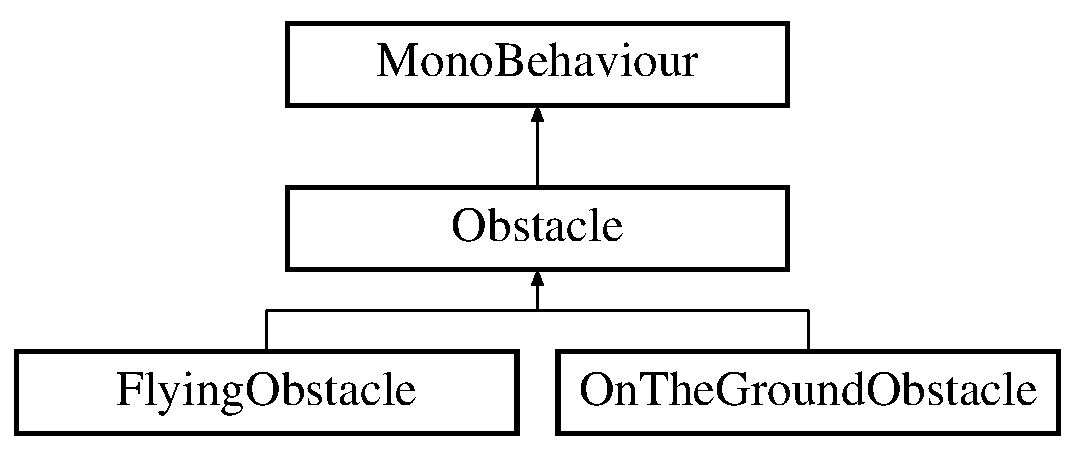
\includegraphics[height=3.000000cm]{class_obstacle}
\end{center}
\end{figure}
\subsection*{Public Member Functions}
\begin{DoxyCompactItemize}
\item 
abstract void \hyperlink{class_obstacle_a19f2f5d2c3176ee9ea8840862c55aa42}{Obstacle\+Maker} ()
\begin{DoxyCompactList}\small\item\em Method abstract pembuat obstacle. \end{DoxyCompactList}\end{DoxyCompactItemize}
\subsection*{Public Attributes}
\begin{DoxyCompactItemize}
\item 
Game\+Object \mbox{[}$\,$\mbox{]} \hyperlink{class_obstacle_a388c8e33dc5a1378f622c048891d0306}{ob}
\begin{DoxyCompactList}\small\item\em Array of obstacle. \end{DoxyCompactList}\item 
Transform \hyperlink{class_obstacle_ad1f3a9f914fb5fbe9367143d8d20ed67}{campos}
\begin{DoxyCompactList}\small\item\em Camera Position. \end{DoxyCompactList}\item 
float \hyperlink{class_obstacle_a84513c71d850ac7c67915fcee2d3df1b}{gap} =1.\+5f
\begin{DoxyCompactList}\small\item\em Gap antar obstacle. \end{DoxyCompactList}\item 
int \hyperlink{class_obstacle_a079bd35101bc96d528ef7246f28de6ea}{obs}
\begin{DoxyCompactList}\small\item\em \hyperlink{class_obstacle}{Obstacle}. \end{DoxyCompactList}\end{DoxyCompactItemize}


\subsection{Detailed Description}
Kelas abstract \hyperlink{class_obstacle}{Obstacle} merepresentasikan obstacle. 



\subsection{Member Function Documentation}
\hypertarget{class_obstacle_a19f2f5d2c3176ee9ea8840862c55aa42}{}\label{class_obstacle_a19f2f5d2c3176ee9ea8840862c55aa42} 
\index{Obstacle@{Obstacle}!Obstacle\+Maker@{Obstacle\+Maker}}
\index{Obstacle\+Maker@{Obstacle\+Maker}!Obstacle@{Obstacle}}
\subsubsection{\texorpdfstring{Obstacle\+Maker()}{ObstacleMaker()}}
{\footnotesize\ttfamily abstract void Obstacle.\+Obstacle\+Maker (\begin{DoxyParamCaption}{ }\end{DoxyParamCaption})\hspace{0.3cm}{\ttfamily [pure virtual]}}



Method abstract pembuat obstacle. 



Implemented in \hyperlink{class_flying_obstacle_a1c21c97ab8d9efa1c120103a2cd5cb34}{Flying\+Obstacle}, and \hyperlink{class_on_the_ground_obstacle_a6c6123b29a6d6c2b78fa12ff72bf0834}{On\+The\+Ground\+Obstacle}.



\subsection{Member Data Documentation}
\hypertarget{class_obstacle_ad1f3a9f914fb5fbe9367143d8d20ed67}{}\label{class_obstacle_ad1f3a9f914fb5fbe9367143d8d20ed67} 
\index{Obstacle@{Obstacle}!campos@{campos}}
\index{campos@{campos}!Obstacle@{Obstacle}}
\subsubsection{\texorpdfstring{campos}{campos}}
{\footnotesize\ttfamily Transform Obstacle.\+campos}



Camera Position. 

\hypertarget{class_obstacle_a84513c71d850ac7c67915fcee2d3df1b}{}\label{class_obstacle_a84513c71d850ac7c67915fcee2d3df1b} 
\index{Obstacle@{Obstacle}!gap@{gap}}
\index{gap@{gap}!Obstacle@{Obstacle}}
\subsubsection{\texorpdfstring{gap}{gap}}
{\footnotesize\ttfamily float Obstacle.\+gap =1.\+5f}



Gap antar obstacle. 

\hypertarget{class_obstacle_a388c8e33dc5a1378f622c048891d0306}{}\label{class_obstacle_a388c8e33dc5a1378f622c048891d0306} 
\index{Obstacle@{Obstacle}!ob@{ob}}
\index{ob@{ob}!Obstacle@{Obstacle}}
\subsubsection{\texorpdfstring{ob}{ob}}
{\footnotesize\ttfamily Game\+Object \mbox{[}$\,$\mbox{]} Obstacle.\+ob}



Array of obstacle. 

\hypertarget{class_obstacle_a079bd35101bc96d528ef7246f28de6ea}{}\label{class_obstacle_a079bd35101bc96d528ef7246f28de6ea} 
\index{Obstacle@{Obstacle}!obs@{obs}}
\index{obs@{obs}!Obstacle@{Obstacle}}
\subsubsection{\texorpdfstring{obs}{obs}}
{\footnotesize\ttfamily int Obstacle.\+obs}



\hyperlink{class_obstacle}{Obstacle}. 



The documentation for this class was generated from the following file\+:\begin{DoxyCompactItemize}
\item 
C\+:/\+Users/\+Public/\+Documents/\+Unity Projects/\+Ellena/\+Ta\+Daa/\+Megaman Endless Run/\+Assets/\+Controller/\+Script/\hyperlink{_obstacle_8cs}{Obstacle.\+cs}\end{DoxyCompactItemize}

\hypertarget{class_on_the_ground_obstacle}{}\section{On\+The\+Ground\+Obstacle Class Reference}
\label{class_on_the_ground_obstacle}\index{On\+The\+Ground\+Obstacle@{On\+The\+Ground\+Obstacle}}


Kelas \hyperlink{class_on_the_ground_obstacle}{On\+The\+Ground\+Obstacle} merepresentasikan obstacle yang berada di atas tanah.  


Inheritance diagram for On\+The\+Ground\+Obstacle\+:\begin{figure}[H]
\begin{center}
\leavevmode
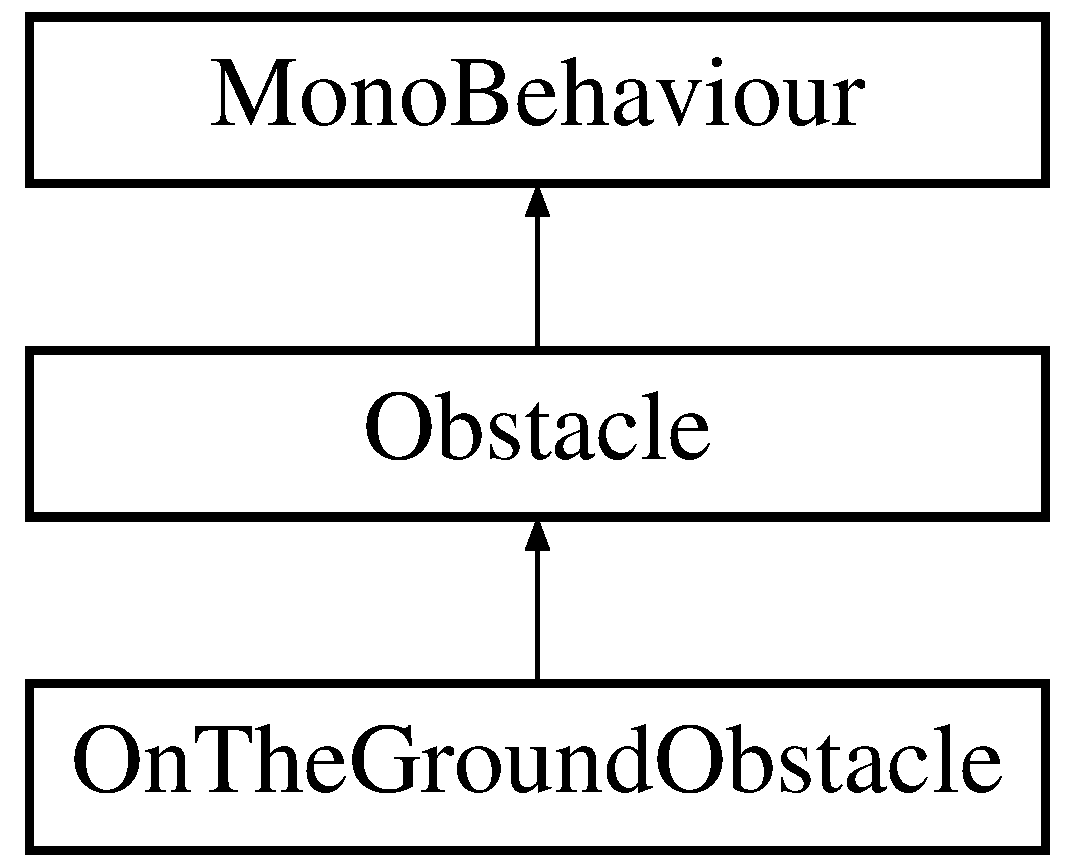
\includegraphics[height=3.000000cm]{class_on_the_ground_obstacle}
\end{center}
\end{figure}
\subsection*{Public Member Functions}
\begin{DoxyCompactItemize}
\item 
override void \hyperlink{class_on_the_ground_obstacle_a6c6123b29a6d6c2b78fa12ff72bf0834}{Obstacle\+Maker} ()
\begin{DoxyCompactList}\small\item\em Membuat \hyperlink{class_obstacle}{Obstacle}. \end{DoxyCompactList}\end{DoxyCompactItemize}
\subsection*{Additional Inherited Members}


\subsection{Detailed Description}
Kelas \hyperlink{class_on_the_ground_obstacle}{On\+The\+Ground\+Obstacle} merepresentasikan obstacle yang berada di atas tanah. 



\subsection{Member Function Documentation}
\hypertarget{class_on_the_ground_obstacle_a6c6123b29a6d6c2b78fa12ff72bf0834}{}\label{class_on_the_ground_obstacle_a6c6123b29a6d6c2b78fa12ff72bf0834} 
\index{On\+The\+Ground\+Obstacle@{On\+The\+Ground\+Obstacle}!Obstacle\+Maker@{Obstacle\+Maker}}
\index{Obstacle\+Maker@{Obstacle\+Maker}!On\+The\+Ground\+Obstacle@{On\+The\+Ground\+Obstacle}}
\subsubsection{\texorpdfstring{Obstacle\+Maker()}{ObstacleMaker()}}
{\footnotesize\ttfamily override void On\+The\+Ground\+Obstacle.\+Obstacle\+Maker (\begin{DoxyParamCaption}{ }\end{DoxyParamCaption})\hspace{0.3cm}{\ttfamily [virtual]}}



Membuat \hyperlink{class_obstacle}{Obstacle}. 



Implements \hyperlink{class_obstacle_a19f2f5d2c3176ee9ea8840862c55aa42}{Obstacle}.



The documentation for this class was generated from the following file\+:\begin{DoxyCompactItemize}
\item 
C\+:/\+Users/\+Public/\+Documents/\+Unity Projects/\+Ellena/\+Ta\+Daa/\+Megaman Endless Run/\+Assets/\+Controller/\+Script/\hyperlink{_on_the_ground_obstacle_8cs}{On\+The\+Ground\+Obstacle.\+cs}\end{DoxyCompactItemize}

\hypertarget{class_preference_controller}{}\section{Preference\+Controller Class Reference}
\label{class_preference_controller}\index{Preference\+Controller@{Preference\+Controller}}


Kelas \hyperlink{class_preference_controller}{Preference\+Controller} mengontrol Preference\+Scene.  


Inheritance diagram for Preference\+Controller\+:\begin{figure}[H]
\begin{center}
\leavevmode
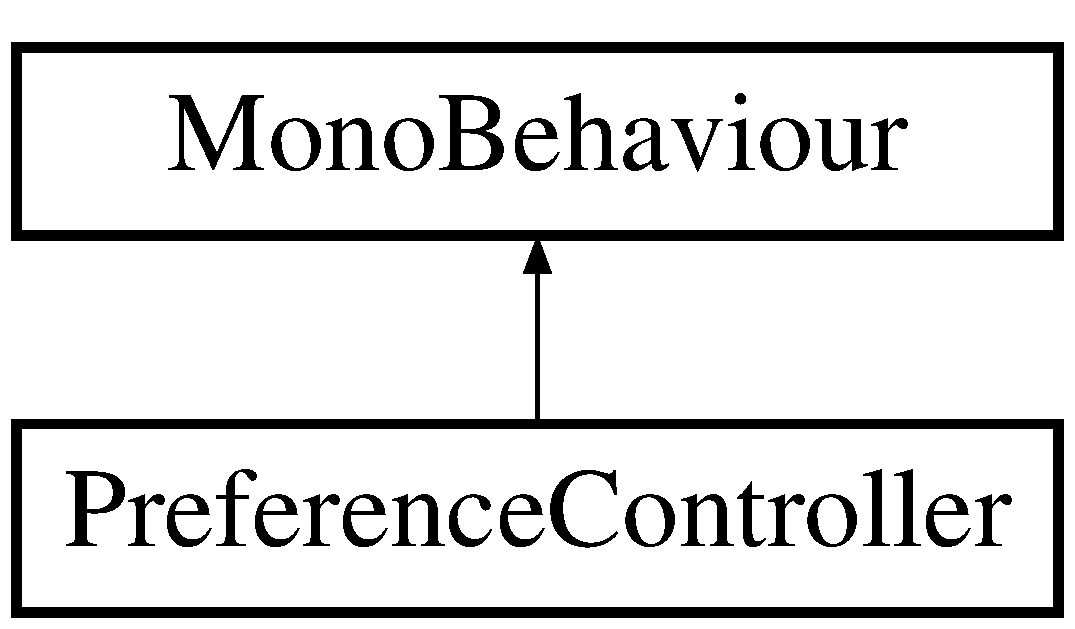
\includegraphics[height=2.000000cm]{class_preference_controller}
\end{center}
\end{figure}
\subsection*{Public Member Functions}
\begin{DoxyCompactItemize}
\item 
void \hyperlink{class_preference_controller_ac1f51dd39b0846f7259bcf2e028cd486}{Volume\+Slider\+Changed} (float new\+Value)
\begin{DoxyCompactList}\small\item\em Mengatur volume suara dengan Volume\+Slider. \end{DoxyCompactList}\item 
void \hyperlink{class_preference_controller_a27079e068e495b9815668db8ceaff04b}{return\+Btn\+On\+Click} ()
\begin{DoxyCompactList}\small\item\em Mengatur tindakan yang dilakukan saat button Return\+Button diklik. Tindakan \+: Kembali ke layar sebelumnya. \end{DoxyCompactList}\end{DoxyCompactItemize}
\subsection*{Public Attributes}
\begin{DoxyCompactItemize}
\item 
Button \hyperlink{class_preference_controller_a1eae6170b41b81919c9ecf14c0ecb86c}{return\+Button}
\begin{DoxyCompactList}\small\item\em Button -\/ button yang ada di Preference\+Scene. \end{DoxyCompactList}\end{DoxyCompactItemize}


\subsection{Detailed Description}
Kelas \hyperlink{class_preference_controller}{Preference\+Controller} mengontrol Preference\+Scene. 



\subsection{Member Function Documentation}
\hypertarget{class_preference_controller_a27079e068e495b9815668db8ceaff04b}{}\label{class_preference_controller_a27079e068e495b9815668db8ceaff04b} 
\index{Preference\+Controller@{Preference\+Controller}!return\+Btn\+On\+Click@{return\+Btn\+On\+Click}}
\index{return\+Btn\+On\+Click@{return\+Btn\+On\+Click}!Preference\+Controller@{Preference\+Controller}}
\subsubsection{\texorpdfstring{return\+Btn\+On\+Click()}{returnBtnOnClick()}}
{\footnotesize\ttfamily void Preference\+Controller.\+return\+Btn\+On\+Click (\begin{DoxyParamCaption}{ }\end{DoxyParamCaption})}



Mengatur tindakan yang dilakukan saat button Return\+Button diklik. Tindakan \+: Kembali ke layar sebelumnya. 

\hypertarget{class_preference_controller_ac1f51dd39b0846f7259bcf2e028cd486}{}\label{class_preference_controller_ac1f51dd39b0846f7259bcf2e028cd486} 
\index{Preference\+Controller@{Preference\+Controller}!Volume\+Slider\+Changed@{Volume\+Slider\+Changed}}
\index{Volume\+Slider\+Changed@{Volume\+Slider\+Changed}!Preference\+Controller@{Preference\+Controller}}
\subsubsection{\texorpdfstring{Volume\+Slider\+Changed()}{VolumeSliderChanged()}}
{\footnotesize\ttfamily void Preference\+Controller.\+Volume\+Slider\+Changed (\begin{DoxyParamCaption}\item[{float}]{new\+Value }\end{DoxyParamCaption})}



Mengatur volume suara dengan Volume\+Slider. 


\begin{DoxyParams}{Parameters}
{\em new\+Value} & New value.\\
\hline
\end{DoxyParams}


\subsection{Member Data Documentation}
\hypertarget{class_preference_controller_a1eae6170b41b81919c9ecf14c0ecb86c}{}\label{class_preference_controller_a1eae6170b41b81919c9ecf14c0ecb86c} 
\index{Preference\+Controller@{Preference\+Controller}!return\+Button@{return\+Button}}
\index{return\+Button@{return\+Button}!Preference\+Controller@{Preference\+Controller}}
\subsubsection{\texorpdfstring{return\+Button}{returnButton}}
{\footnotesize\ttfamily Button Preference\+Controller.\+return\+Button}



Button -\/ button yang ada di Preference\+Scene. 



The documentation for this class was generated from the following file\+:\begin{DoxyCompactItemize}
\item 
C\+:/\+Users/\+Public/\+Documents/\+Unity Projects/\+Ellena/\+Ta\+Daa/\+Megaman Endless Run/\+Assets/\+Controller/\+Script/\hyperlink{_preference_controller_8cs}{Preference\+Controller.\+cs}\end{DoxyCompactItemize}

\hypertarget{class_quit_controller}{}\section{Quit\+Controller Class Reference}
\label{class_quit_controller}\index{Quit\+Controller@{Quit\+Controller}}


Kelas \hyperlink{class_quit_controller}{Quit\+Controller} mengontrol Quit\+Scene.  


Inheritance diagram for Quit\+Controller\+:\begin{figure}[H]
\begin{center}
\leavevmode
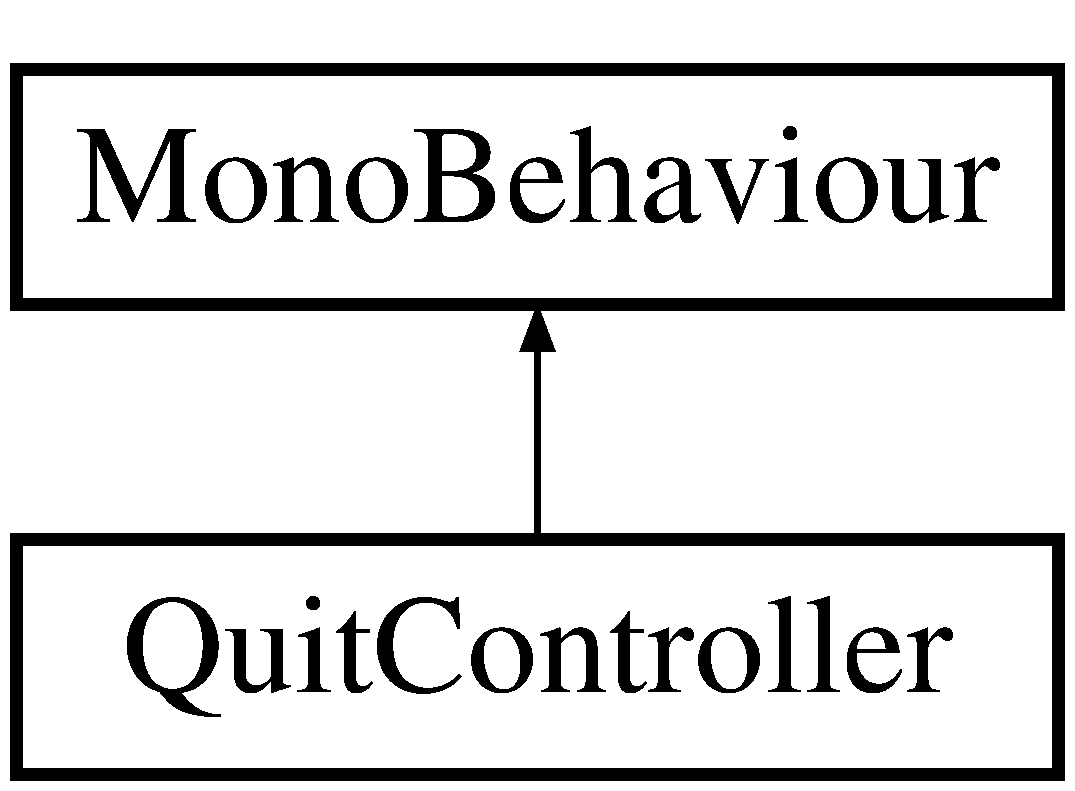
\includegraphics[height=2.000000cm]{class_quit_controller}
\end{center}
\end{figure}
\subsection*{Public Member Functions}
\begin{DoxyCompactItemize}
\item 
void \hyperlink{class_quit_controller_a3f4f0e9b67108e4a0608f4c2085cac84}{yes\+Btn\+On\+Click} ()
\begin{DoxyCompactList}\small\item\em Mengatur tindakan yang dilakukan saat button Yes\+Button diklik. Tindakan \+: Keluar dari game. \end{DoxyCompactList}\item 
void \hyperlink{class_quit_controller_aa0339f4778f5e947a0f1a041734757f0}{no\+Btn\+On\+Click} ()
\begin{DoxyCompactList}\small\item\em Mengatur tindakan yang dilakukan saat button No\+Button diklik. Tindakan \+: Kembali ke layar sebelumnya. \end{DoxyCompactList}\end{DoxyCompactItemize}
\subsection*{Public Attributes}
\begin{DoxyCompactItemize}
\item 
Button \hyperlink{class_quit_controller_a988a4085bd05debd186ee7475e758404}{Yes\+Button}
\begin{DoxyCompactList}\small\item\em Button -\/ button yang ada di Quit\+Scene. \end{DoxyCompactList}\end{DoxyCompactItemize}


\subsection{Detailed Description}
Kelas \hyperlink{class_quit_controller}{Quit\+Controller} mengontrol Quit\+Scene. 



\subsection{Member Function Documentation}
\hypertarget{class_quit_controller_aa0339f4778f5e947a0f1a041734757f0}{}\label{class_quit_controller_aa0339f4778f5e947a0f1a041734757f0} 
\index{Quit\+Controller@{Quit\+Controller}!no\+Btn\+On\+Click@{no\+Btn\+On\+Click}}
\index{no\+Btn\+On\+Click@{no\+Btn\+On\+Click}!Quit\+Controller@{Quit\+Controller}}
\subsubsection{\texorpdfstring{no\+Btn\+On\+Click()}{noBtnOnClick()}}
{\footnotesize\ttfamily void Quit\+Controller.\+no\+Btn\+On\+Click (\begin{DoxyParamCaption}{ }\end{DoxyParamCaption})}



Mengatur tindakan yang dilakukan saat button No\+Button diklik. Tindakan \+: Kembali ke layar sebelumnya. 

\hypertarget{class_quit_controller_a3f4f0e9b67108e4a0608f4c2085cac84}{}\label{class_quit_controller_a3f4f0e9b67108e4a0608f4c2085cac84} 
\index{Quit\+Controller@{Quit\+Controller}!yes\+Btn\+On\+Click@{yes\+Btn\+On\+Click}}
\index{yes\+Btn\+On\+Click@{yes\+Btn\+On\+Click}!Quit\+Controller@{Quit\+Controller}}
\subsubsection{\texorpdfstring{yes\+Btn\+On\+Click()}{yesBtnOnClick()}}
{\footnotesize\ttfamily void Quit\+Controller.\+yes\+Btn\+On\+Click (\begin{DoxyParamCaption}{ }\end{DoxyParamCaption})}



Mengatur tindakan yang dilakukan saat button Yes\+Button diklik. Tindakan \+: Keluar dari game. 



\subsection{Member Data Documentation}
\hypertarget{class_quit_controller_a988a4085bd05debd186ee7475e758404}{}\label{class_quit_controller_a988a4085bd05debd186ee7475e758404} 
\index{Quit\+Controller@{Quit\+Controller}!Yes\+Button@{Yes\+Button}}
\index{Yes\+Button@{Yes\+Button}!Quit\+Controller@{Quit\+Controller}}
\subsubsection{\texorpdfstring{Yes\+Button}{YesButton}}
{\footnotesize\ttfamily Button Quit\+Controller.\+Yes\+Button}



Button -\/ button yang ada di Quit\+Scene. 



The documentation for this class was generated from the following file\+:\begin{DoxyCompactItemize}
\item 
C\+:/\+Users/\+Public/\+Documents/\+Unity Projects/\+Ellena/\+Ta\+Daa/\+Megaman Endless Run/\+Assets/\+Controller/\+Script/\hyperlink{_quit_controller_8cs}{Quit\+Controller.\+cs}\end{DoxyCompactItemize}

\hypertarget{class_runner}{}\section{Runner Class Reference}
\label{class_runner}\index{Runner@{Runner}}


Kelas \hyperlink{class_runner}{Runner} merepresentasikan runner.  


Inheritance diagram for Runner\+:\begin{figure}[H]
\begin{center}
\leavevmode
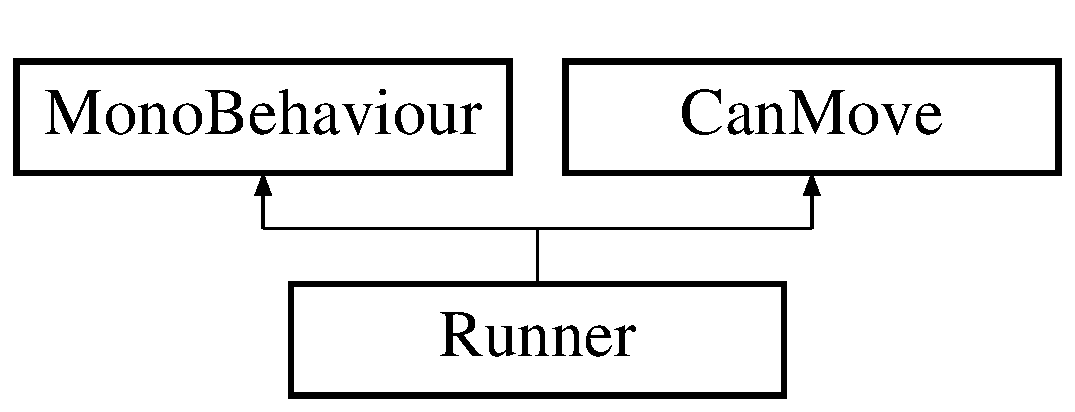
\includegraphics[height=2.000000cm]{class_runner}
\end{center}
\end{figure}
\subsection*{Public Member Functions}
\begin{DoxyCompactItemize}
\item 
void \hyperlink{class_runner_add0c89849fa2e023ed488ba80c7daf4a}{Move} ()
\begin{DoxyCompactList}\small\item\em menggerakan character sesuai input pemain. \end{DoxyCompactList}\end{DoxyCompactItemize}
\subsection*{Public Attributes}
\begin{DoxyCompactItemize}
\item 
Audio\+Source \hyperlink{class_runner_a7480846642a3f6ed85a33479d93a46eb}{sound\+F\+X\+Jump}
\begin{DoxyCompactList}\small\item\em Atribut yang akan diisikan audio source dari unity. \end{DoxyCompactList}\end{DoxyCompactItemize}


\subsection{Detailed Description}
Kelas \hyperlink{class_runner}{Runner} merepresentasikan runner. 



\subsection{Member Function Documentation}
\hypertarget{class_runner_add0c89849fa2e023ed488ba80c7daf4a}{}\label{class_runner_add0c89849fa2e023ed488ba80c7daf4a} 
\index{Runner@{Runner}!Move@{Move}}
\index{Move@{Move}!Runner@{Runner}}
\subsubsection{\texorpdfstring{Move()}{Move()}}
{\footnotesize\ttfamily void Runner.\+Move (\begin{DoxyParamCaption}{ }\end{DoxyParamCaption})}



menggerakan character sesuai input pemain. 



Implements \hyperlink{interface_can_move_a2c40a4dc4684e8f04e31ff59d4ec74e0}{Can\+Move}.



\subsection{Member Data Documentation}
\hypertarget{class_runner_a7480846642a3f6ed85a33479d93a46eb}{}\label{class_runner_a7480846642a3f6ed85a33479d93a46eb} 
\index{Runner@{Runner}!sound\+F\+X\+Jump@{sound\+F\+X\+Jump}}
\index{sound\+F\+X\+Jump@{sound\+F\+X\+Jump}!Runner@{Runner}}
\subsubsection{\texorpdfstring{sound\+F\+X\+Jump}{soundFXJump}}
{\footnotesize\ttfamily Audio\+Source Runner.\+sound\+F\+X\+Jump}



Atribut yang akan diisikan audio source dari unity. 



The documentation for this class was generated from the following file\+:\begin{DoxyCompactItemize}
\item 
C\+:/\+Users/\+Public/\+Documents/\+Unity Projects/\+Ellena/\+Ta\+Daa/\+Megaman Endless Run/\+Assets/\+View/\+Script/\hyperlink{_runner_8cs}{Runner.\+cs}\end{DoxyCompactItemize}

\hypertarget{class_siang_malam}{}\section{Siang\+Malam Class Reference}
\label{class_siang_malam}\index{Siang\+Malam@{Siang\+Malam}}


Kelas \hyperlink{class_siang_malam}{Siang\+Malam} mengatur siang malam di gamr.  


Inheritance diagram for Siang\+Malam\+:\begin{figure}[H]
\begin{center}
\leavevmode
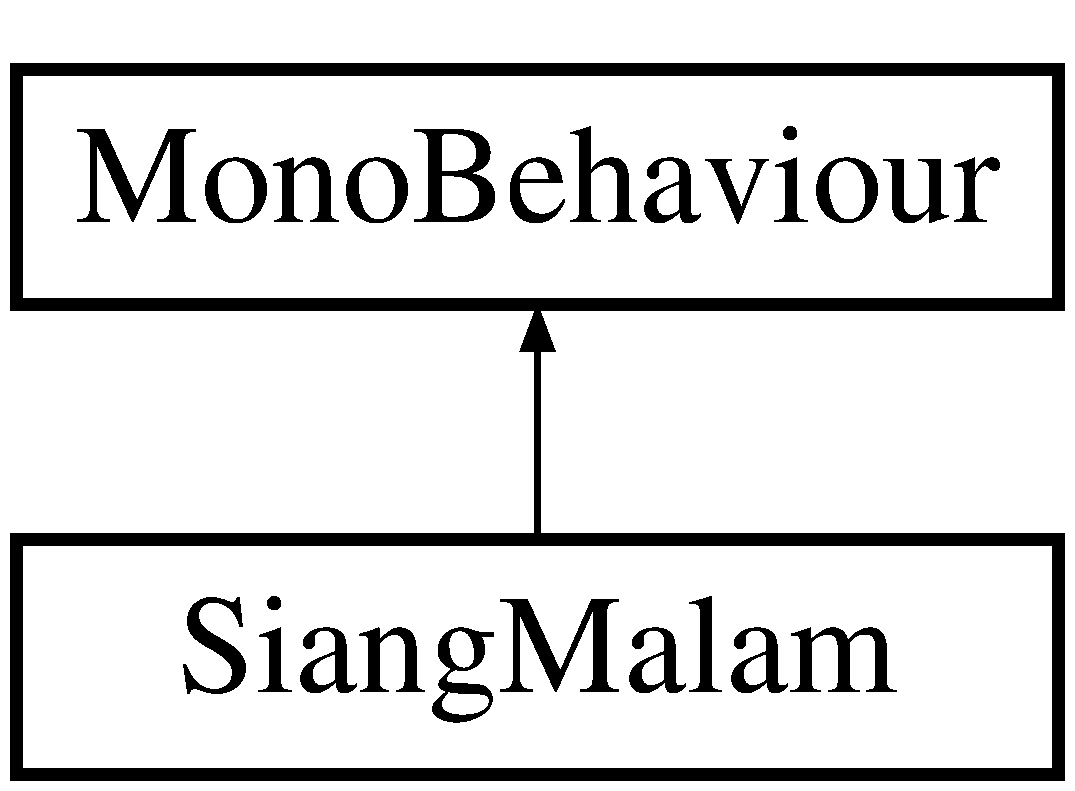
\includegraphics[height=2.000000cm]{class_siang_malam}
\end{center}
\end{figure}
\subsection*{Public Member Functions}
\begin{DoxyCompactItemize}
\item 
void \hyperlink{class_siang_malam_a1fccd6abbcae495a27af288d2aabf9a6}{Ubah\+X\+Bulan} ()
\begin{DoxyCompactList}\small\item\em Memutar posisi bulan. \end{DoxyCompactList}\end{DoxyCompactItemize}
\subsection*{Public Attributes}
\begin{DoxyCompactItemize}
\item 
Shader \hyperlink{class_siang_malam_a0178556607a805c0d69f623512bb1bf5}{H\+S\+V\+Shader}
\begin{DoxyCompactList}\small\item\em The H\+SV shader. \end{DoxyCompactList}\item 
bool \hyperlink{class_siang_malam_af85d640c6eebc35947063e0df9595794}{siang} = true
\begin{DoxyCompactList}\small\item\em true = siang, false = malam. \end{DoxyCompactList}\item 
Game\+Object \hyperlink{class_siang_malam_a28d5bb8091f1f0160959fce37bdafccd}{ob1}
\begin{DoxyCompactList}\small\item\em Object game 1. \end{DoxyCompactList}\item 
Game\+Object \hyperlink{class_siang_malam_ac903e5559288c82b9767674461899742}{ob2}
\begin{DoxyCompactList}\small\item\em Object game 2. \end{DoxyCompactList}\item 
Game\+Object \hyperlink{class_siang_malam_a1a1e6645cb6a9e4cfa6d753a5c10cfcf}{bulan}
\begin{DoxyCompactList}\small\item\em Bulan. \end{DoxyCompactList}\item 
Sprite \mbox{[}$\,$\mbox{]} \hyperlink{class_siang_malam_a2d931b869867f22ed03b106d66868354}{bulan\+Sprites}
\begin{DoxyCompactList}\small\item\em Sprites bulan. \end{DoxyCompactList}\end{DoxyCompactItemize}


\subsection{Detailed Description}
Kelas \hyperlink{class_siang_malam}{Siang\+Malam} mengatur siang malam di gamr. 



\subsection{Member Function Documentation}
\hypertarget{class_siang_malam_a1fccd6abbcae495a27af288d2aabf9a6}{}\label{class_siang_malam_a1fccd6abbcae495a27af288d2aabf9a6} 
\index{Siang\+Malam@{Siang\+Malam}!Ubah\+X\+Bulan@{Ubah\+X\+Bulan}}
\index{Ubah\+X\+Bulan@{Ubah\+X\+Bulan}!Siang\+Malam@{Siang\+Malam}}
\subsubsection{\texorpdfstring{Ubah\+X\+Bulan()}{UbahXBulan()}}
{\footnotesize\ttfamily void Siang\+Malam.\+Ubah\+X\+Bulan (\begin{DoxyParamCaption}{ }\end{DoxyParamCaption})}



Memutar posisi bulan. 



\subsection{Member Data Documentation}
\hypertarget{class_siang_malam_a1a1e6645cb6a9e4cfa6d753a5c10cfcf}{}\label{class_siang_malam_a1a1e6645cb6a9e4cfa6d753a5c10cfcf} 
\index{Siang\+Malam@{Siang\+Malam}!bulan@{bulan}}
\index{bulan@{bulan}!Siang\+Malam@{Siang\+Malam}}
\subsubsection{\texorpdfstring{bulan}{bulan}}
{\footnotesize\ttfamily Game\+Object Siang\+Malam.\+bulan}



Bulan. 

\hypertarget{class_siang_malam_a2d931b869867f22ed03b106d66868354}{}\label{class_siang_malam_a2d931b869867f22ed03b106d66868354} 
\index{Siang\+Malam@{Siang\+Malam}!bulan\+Sprites@{bulan\+Sprites}}
\index{bulan\+Sprites@{bulan\+Sprites}!Siang\+Malam@{Siang\+Malam}}
\subsubsection{\texorpdfstring{bulan\+Sprites}{bulanSprites}}
{\footnotesize\ttfamily Sprite \mbox{[}$\,$\mbox{]} Siang\+Malam.\+bulan\+Sprites}



Sprites bulan. 

\hypertarget{class_siang_malam_a0178556607a805c0d69f623512bb1bf5}{}\label{class_siang_malam_a0178556607a805c0d69f623512bb1bf5} 
\index{Siang\+Malam@{Siang\+Malam}!H\+S\+V\+Shader@{H\+S\+V\+Shader}}
\index{H\+S\+V\+Shader@{H\+S\+V\+Shader}!Siang\+Malam@{Siang\+Malam}}
\subsubsection{\texorpdfstring{H\+S\+V\+Shader}{HSVShader}}
{\footnotesize\ttfamily Shader Siang\+Malam.\+H\+S\+V\+Shader}



The H\+SV shader. 

\hypertarget{class_siang_malam_a28d5bb8091f1f0160959fce37bdafccd}{}\label{class_siang_malam_a28d5bb8091f1f0160959fce37bdafccd} 
\index{Siang\+Malam@{Siang\+Malam}!ob1@{ob1}}
\index{ob1@{ob1}!Siang\+Malam@{Siang\+Malam}}
\subsubsection{\texorpdfstring{ob1}{ob1}}
{\footnotesize\ttfamily Game\+Object Siang\+Malam.\+ob1}



Object game 1. 

\hypertarget{class_siang_malam_ac903e5559288c82b9767674461899742}{}\label{class_siang_malam_ac903e5559288c82b9767674461899742} 
\index{Siang\+Malam@{Siang\+Malam}!ob2@{ob2}}
\index{ob2@{ob2}!Siang\+Malam@{Siang\+Malam}}
\subsubsection{\texorpdfstring{ob2}{ob2}}
{\footnotesize\ttfamily Game\+Object Siang\+Malam.\+ob2}



Object game 2. 

\hypertarget{class_siang_malam_af85d640c6eebc35947063e0df9595794}{}\label{class_siang_malam_af85d640c6eebc35947063e0df9595794} 
\index{Siang\+Malam@{Siang\+Malam}!siang@{siang}}
\index{siang@{siang}!Siang\+Malam@{Siang\+Malam}}
\subsubsection{\texorpdfstring{siang}{siang}}
{\footnotesize\ttfamily bool Siang\+Malam.\+siang = true}



true = siang, false = malam. 



The documentation for this class was generated from the following file\+:\begin{DoxyCompactItemize}
\item 
C\+:/\+Users/\+Public/\+Documents/\+Unity Projects/\+Ellena/\+Ta\+Daa/\+Megaman Endless Run/\+Assets/\+View/\+Script/\hyperlink{_siang_malam_8cs}{Siang\+Malam.\+cs}\end{DoxyCompactItemize}

\hypertarget{class_sounds_controller}{}\section{Sounds\+Controller Class Reference}
\label{class_sounds_controller}\index{Sounds\+Controller@{Sounds\+Controller}}


Kelas Sounds controller mengontrol suara pada game.  


Inheritance diagram for Sounds\+Controller\+:\begin{figure}[H]
\begin{center}
\leavevmode
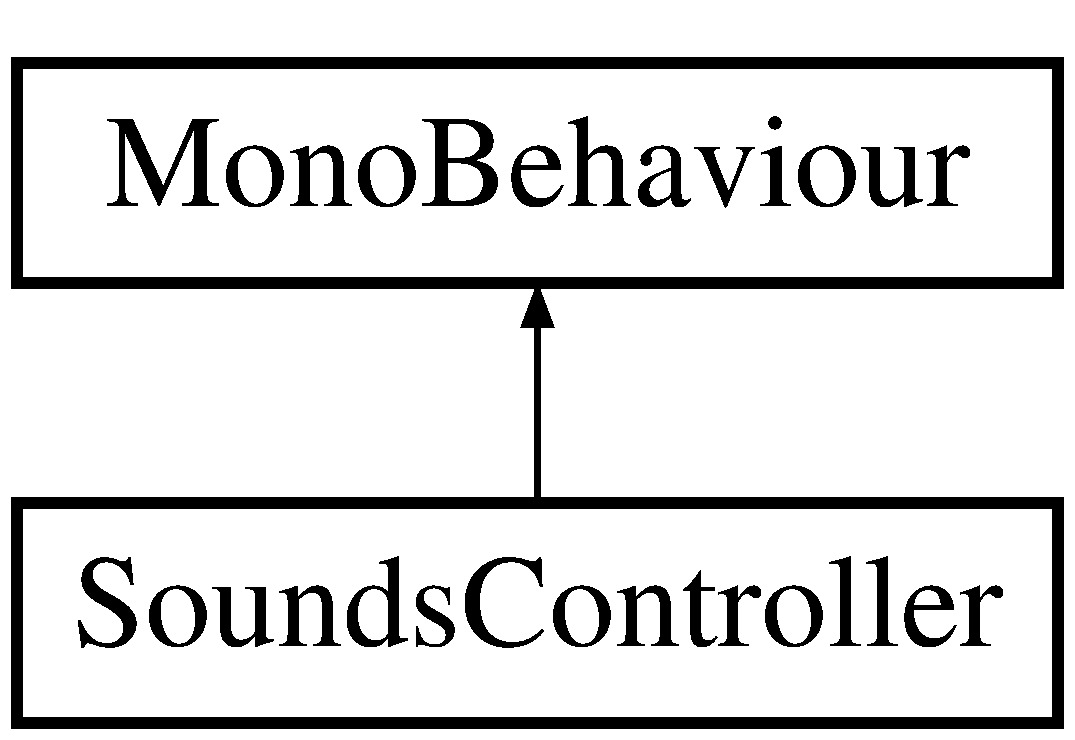
\includegraphics[height=2.000000cm]{class_sounds_controller}
\end{center}
\end{figure}


\subsection{Detailed Description}
Kelas Sounds controller mengontrol suara pada game. 



The documentation for this class was generated from the following file\+:\begin{DoxyCompactItemize}
\item 
C\+:/\+Users/\+Public/\+Documents/\+Unity Projects/\+Ellena/\+Ta\+Daa/\+Megaman Endless Run/\+Assets/\+Controller/\+Script/\hyperlink{_sounds_controller_8cs}{Sounds\+Controller.\+cs}\end{DoxyCompactItemize}

\chapter{File Documentation}
\hypertarget{_credit_controller_8cs}{}\section{C\+:/\+Users/\+Public/\+Documents/\+Unity Projects/\+Ellena/\+Ta\+Daa/\+Megaman Endless Run/\+Assets/\+Controller/\+Script/\+Credit\+Controller.cs File Reference}
\label{_credit_controller_8cs}\index{C\+:/\+Users/\+Public/\+Documents/\+Unity Projects/\+Ellena/\+Ta\+Daa/\+Megaman Endless Run/\+Assets/\+Controller/\+Script/\+Credit\+Controller.\+cs@{C\+:/\+Users/\+Public/\+Documents/\+Unity Projects/\+Ellena/\+Ta\+Daa/\+Megaman Endless Run/\+Assets/\+Controller/\+Script/\+Credit\+Controller.\+cs}}
\subsection*{Classes}
\begin{DoxyCompactItemize}
\item 
class \hyperlink{class_credit_controller}{Credit\+Controller}
\begin{DoxyCompactList}\small\item\em Kelas \hyperlink{class_credit_controller}{Credit\+Controller} mengontrol Credit\+Scene. \end{DoxyCompactList}\end{DoxyCompactItemize}

\hypertarget{_flying_obstacle_8cs}{}\section{C\+:/\+Users/\+Public/\+Documents/\+Unity Projects/\+Ellena/\+Ta\+Daa/\+Megaman Endless Run/\+Assets/\+Controller/\+Script/\+Flying\+Obstacle.cs File Reference}
\label{_flying_obstacle_8cs}\index{C\+:/\+Users/\+Public/\+Documents/\+Unity Projects/\+Ellena/\+Ta\+Daa/\+Megaman Endless Run/\+Assets/\+Controller/\+Script/\+Flying\+Obstacle.\+cs@{C\+:/\+Users/\+Public/\+Documents/\+Unity Projects/\+Ellena/\+Ta\+Daa/\+Megaman Endless Run/\+Assets/\+Controller/\+Script/\+Flying\+Obstacle.\+cs}}
\subsection*{Classes}
\begin{DoxyCompactItemize}
\item 
class \hyperlink{class_flying_obstacle}{Flying\+Obstacle}
\begin{DoxyCompactList}\small\item\em Kelas \hyperlink{class_flying_obstacle}{Flying\+Obstacle} merepresentasikan obstacle yang dapat terbang. \end{DoxyCompactList}\end{DoxyCompactItemize}

\hypertarget{_game_over_8cs}{}\section{C\+:/\+Users/\+Public/\+Documents/\+Unity Projects/\+Ellena/\+Ta\+Daa/\+Megaman Endless Run/\+Assets/\+Controller/\+Script/\+Game\+Over.cs File Reference}
\label{_game_over_8cs}\index{C\+:/\+Users/\+Public/\+Documents/\+Unity Projects/\+Ellena/\+Ta\+Daa/\+Megaman Endless Run/\+Assets/\+Controller/\+Script/\+Game\+Over.\+cs@{C\+:/\+Users/\+Public/\+Documents/\+Unity Projects/\+Ellena/\+Ta\+Daa/\+Megaman Endless Run/\+Assets/\+Controller/\+Script/\+Game\+Over.\+cs}}
\subsection*{Classes}
\begin{DoxyCompactItemize}
\item 
class \hyperlink{class_game_over}{Game\+Over}
\begin{DoxyCompactList}\small\item\em Kelas \hyperlink{class_game_over}{Game\+Over} merepresentasikan game saat game over. \end{DoxyCompactList}\end{DoxyCompactItemize}

\hypertarget{_main_menu_controller_8cs}{}\section{C\+:/\+Users/\+Public/\+Documents/\+Unity Projects/\+Ellena/\+Ta\+Daa/\+Megaman Endless Run/\+Assets/\+Controller/\+Script/\+Main\+Menu\+Controller.cs File Reference}
\label{_main_menu_controller_8cs}\index{C\+:/\+Users/\+Public/\+Documents/\+Unity Projects/\+Ellena/\+Ta\+Daa/\+Megaman Endless Run/\+Assets/\+Controller/\+Script/\+Main\+Menu\+Controller.\+cs@{C\+:/\+Users/\+Public/\+Documents/\+Unity Projects/\+Ellena/\+Ta\+Daa/\+Megaman Endless Run/\+Assets/\+Controller/\+Script/\+Main\+Menu\+Controller.\+cs}}
\subsection*{Classes}
\begin{DoxyCompactItemize}
\item 
class \hyperlink{class_main_menu_controller}{Main\+Menu\+Controller}
\begin{DoxyCompactList}\small\item\em Kelas \hyperlink{class_main_menu_controller}{Main\+Menu\+Controller} mengontrol Main\+Menu\+Scene. \end{DoxyCompactList}\end{DoxyCompactItemize}

\hypertarget{_obstacle_8cs}{}\section{C\+:/\+Users/\+Public/\+Documents/\+Unity Projects/\+Ellena/\+Ta\+Daa/\+Megaman Endless Run/\+Assets/\+Controller/\+Script/\+Obstacle.cs File Reference}
\label{_obstacle_8cs}\index{C\+:/\+Users/\+Public/\+Documents/\+Unity Projects/\+Ellena/\+Ta\+Daa/\+Megaman Endless Run/\+Assets/\+Controller/\+Script/\+Obstacle.\+cs@{C\+:/\+Users/\+Public/\+Documents/\+Unity Projects/\+Ellena/\+Ta\+Daa/\+Megaman Endless Run/\+Assets/\+Controller/\+Script/\+Obstacle.\+cs}}
\subsection*{Classes}
\begin{DoxyCompactItemize}
\item 
class \hyperlink{class_obstacle}{Obstacle}
\begin{DoxyCompactList}\small\item\em Kelas abstract \hyperlink{class_obstacle}{Obstacle} merepresentasikan obstacle. \end{DoxyCompactList}\end{DoxyCompactItemize}

\hypertarget{_on_the_ground_obstacle_8cs}{}\section{C\+:/\+Users/\+Public/\+Documents/\+Unity Projects/\+Ellena/\+Ta\+Daa/\+Megaman Endless Run/\+Assets/\+Controller/\+Script/\+On\+The\+Ground\+Obstacle.cs File Reference}
\label{_on_the_ground_obstacle_8cs}\index{C\+:/\+Users/\+Public/\+Documents/\+Unity Projects/\+Ellena/\+Ta\+Daa/\+Megaman Endless Run/\+Assets/\+Controller/\+Script/\+On\+The\+Ground\+Obstacle.\+cs@{C\+:/\+Users/\+Public/\+Documents/\+Unity Projects/\+Ellena/\+Ta\+Daa/\+Megaman Endless Run/\+Assets/\+Controller/\+Script/\+On\+The\+Ground\+Obstacle.\+cs}}
\subsection*{Classes}
\begin{DoxyCompactItemize}
\item 
class \hyperlink{class_on_the_ground_obstacle}{On\+The\+Ground\+Obstacle}
\begin{DoxyCompactList}\small\item\em Kelas \hyperlink{class_on_the_ground_obstacle}{On\+The\+Ground\+Obstacle} merepresentasikan obstacle yang berada di atas tanah. \end{DoxyCompactList}\end{DoxyCompactItemize}

\hypertarget{_preference_controller_8cs}{}\section{C\+:/\+Users/\+Public/\+Documents/\+Unity Projects/\+Ellena/\+Ta\+Daa/\+Megaman Endless Run/\+Assets/\+Controller/\+Script/\+Preference\+Controller.cs File Reference}
\label{_preference_controller_8cs}\index{C\+:/\+Users/\+Public/\+Documents/\+Unity Projects/\+Ellena/\+Ta\+Daa/\+Megaman Endless Run/\+Assets/\+Controller/\+Script/\+Preference\+Controller.\+cs@{C\+:/\+Users/\+Public/\+Documents/\+Unity Projects/\+Ellena/\+Ta\+Daa/\+Megaman Endless Run/\+Assets/\+Controller/\+Script/\+Preference\+Controller.\+cs}}
\subsection*{Classes}
\begin{DoxyCompactItemize}
\item 
class \hyperlink{class_preference_controller}{Preference\+Controller}
\begin{DoxyCompactList}\small\item\em Kelas \hyperlink{class_preference_controller}{Preference\+Controller} mengontrol Preference\+Scene. \end{DoxyCompactList}\end{DoxyCompactItemize}

\hypertarget{_quit_controller_8cs}{}\section{C\+:/\+Users/\+Public/\+Documents/\+Unity Projects/\+Ellena/\+Ta\+Daa/\+Megaman Endless Run/\+Assets/\+Controller/\+Script/\+Quit\+Controller.cs File Reference}
\label{_quit_controller_8cs}\index{C\+:/\+Users/\+Public/\+Documents/\+Unity Projects/\+Ellena/\+Ta\+Daa/\+Megaman Endless Run/\+Assets/\+Controller/\+Script/\+Quit\+Controller.\+cs@{C\+:/\+Users/\+Public/\+Documents/\+Unity Projects/\+Ellena/\+Ta\+Daa/\+Megaman Endless Run/\+Assets/\+Controller/\+Script/\+Quit\+Controller.\+cs}}
\subsection*{Classes}
\begin{DoxyCompactItemize}
\item 
class \hyperlink{class_quit_controller}{Quit\+Controller}
\begin{DoxyCompactList}\small\item\em Kelas \hyperlink{class_quit_controller}{Quit\+Controller} mengontrol Quit\+Scene. \end{DoxyCompactList}\end{DoxyCompactItemize}

\hypertarget{_sounds_controller_8cs}{}\section{C\+:/\+Users/\+Public/\+Documents/\+Unity Projects/\+Ellena/\+Ta\+Daa/\+Megaman Endless Run/\+Assets/\+Controller/\+Script/\+Sounds\+Controller.cs File Reference}
\label{_sounds_controller_8cs}\index{C\+:/\+Users/\+Public/\+Documents/\+Unity Projects/\+Ellena/\+Ta\+Daa/\+Megaman Endless Run/\+Assets/\+Controller/\+Script/\+Sounds\+Controller.\+cs@{C\+:/\+Users/\+Public/\+Documents/\+Unity Projects/\+Ellena/\+Ta\+Daa/\+Megaman Endless Run/\+Assets/\+Controller/\+Script/\+Sounds\+Controller.\+cs}}
\subsection*{Classes}
\begin{DoxyCompactItemize}
\item 
class \hyperlink{class_sounds_controller}{Sounds\+Controller}
\begin{DoxyCompactList}\small\item\em Kelas Sounds controller mengontrol suara pada game. \end{DoxyCompactList}\end{DoxyCompactItemize}

\hypertarget{_can_move_8cs}{}\section{C\+:/\+Users/\+Public/\+Documents/\+Unity Projects/\+Ellena/\+Ta\+Daa/\+Megaman Endless Run/\+Assets/\+Model/\+Script/\+Can\+Move.cs File Reference}
\label{_can_move_8cs}\index{C\+:/\+Users/\+Public/\+Documents/\+Unity Projects/\+Ellena/\+Ta\+Daa/\+Megaman Endless Run/\+Assets/\+Model/\+Script/\+Can\+Move.\+cs@{C\+:/\+Users/\+Public/\+Documents/\+Unity Projects/\+Ellena/\+Ta\+Daa/\+Megaman Endless Run/\+Assets/\+Model/\+Script/\+Can\+Move.\+cs}}
\subsection*{Classes}
\begin{DoxyCompactItemize}
\item 
interface \hyperlink{interface_can_move}{Can\+Move}
\end{DoxyCompactItemize}

\hypertarget{_high_score_8cs}{}\section{C\+:/\+Users/\+Public/\+Documents/\+Unity Projects/\+Ellena/\+Ta\+Daa/\+Megaman Endless Run/\+Assets/\+Model/\+Script/\+High\+Score.cs File Reference}
\label{_high_score_8cs}\index{C\+:/\+Users/\+Public/\+Documents/\+Unity Projects/\+Ellena/\+Ta\+Daa/\+Megaman Endless Run/\+Assets/\+Model/\+Script/\+High\+Score.\+cs@{C\+:/\+Users/\+Public/\+Documents/\+Unity Projects/\+Ellena/\+Ta\+Daa/\+Megaman Endless Run/\+Assets/\+Model/\+Script/\+High\+Score.\+cs}}
\subsection*{Classes}
\begin{DoxyCompactItemize}
\item 
class \hyperlink{class_high_score_script}{High\+Score\+Script}
\end{DoxyCompactItemize}

\hypertarget{_back_ground_8cs}{}\section{C\+:/\+Users/\+Public/\+Documents/\+Unity Projects/\+Ellena/\+Ta\+Daa/\+Megaman Endless Run/\+Assets/\+View/\+Script/\+Back\+Ground.cs File Reference}
\label{_back_ground_8cs}\index{C\+:/\+Users/\+Public/\+Documents/\+Unity Projects/\+Ellena/\+Ta\+Daa/\+Megaman Endless Run/\+Assets/\+View/\+Script/\+Back\+Ground.\+cs@{C\+:/\+Users/\+Public/\+Documents/\+Unity Projects/\+Ellena/\+Ta\+Daa/\+Megaman Endless Run/\+Assets/\+View/\+Script/\+Back\+Ground.\+cs}}
\subsection*{Classes}
\begin{DoxyCompactItemize}
\item 
class \hyperlink{class_back_ground}{Back\+Ground}
\begin{DoxyCompactList}\small\item\em Kelas \hyperlink{class_back_ground}{Back\+Ground} mengatur background pada Game\+Scene. \end{DoxyCompactList}\end{DoxyCompactItemize}

\hypertarget{_game_controller_8cs}{}\section{C\+:/\+Users/\+Public/\+Documents/\+Unity Projects/\+Ellena/\+Ta\+Daa/\+Megaman Endless Run/\+Assets/\+View/\+Script/\+Game\+Controller.cs File Reference}
\label{_game_controller_8cs}\index{C\+:/\+Users/\+Public/\+Documents/\+Unity Projects/\+Ellena/\+Ta\+Daa/\+Megaman Endless Run/\+Assets/\+View/\+Script/\+Game\+Controller.\+cs@{C\+:/\+Users/\+Public/\+Documents/\+Unity Projects/\+Ellena/\+Ta\+Daa/\+Megaman Endless Run/\+Assets/\+View/\+Script/\+Game\+Controller.\+cs}}
\subsection*{Classes}
\begin{DoxyCompactItemize}
\item 
class \hyperlink{class_game_controller}{Game\+Controller}
\begin{DoxyCompactList}\small\item\em Kelas \hyperlink{class_game_controller}{Game\+Controller} mengatur score game. \end{DoxyCompactList}\end{DoxyCompactItemize}

\hypertarget{_runner_8cs}{}\section{C\+:/\+Users/\+Public/\+Documents/\+Unity Projects/\+Ellena/\+Ta\+Daa/\+Megaman Endless Run/\+Assets/\+View/\+Script/\+Runner.cs File Reference}
\label{_runner_8cs}\index{C\+:/\+Users/\+Public/\+Documents/\+Unity Projects/\+Ellena/\+Ta\+Daa/\+Megaman Endless Run/\+Assets/\+View/\+Script/\+Runner.\+cs@{C\+:/\+Users/\+Public/\+Documents/\+Unity Projects/\+Ellena/\+Ta\+Daa/\+Megaman Endless Run/\+Assets/\+View/\+Script/\+Runner.\+cs}}
\subsection*{Classes}
\begin{DoxyCompactItemize}
\item 
class \hyperlink{class_runner}{Runner}
\begin{DoxyCompactList}\small\item\em Kelas \hyperlink{class_runner}{Runner} merepresentasikan runner. \end{DoxyCompactList}\end{DoxyCompactItemize}

\hypertarget{_siang_malam_8cs}{}\section{C\+:/\+Users/\+Public/\+Documents/\+Unity Projects/\+Ellena/\+Ta\+Daa/\+Megaman Endless Run/\+Assets/\+View/\+Script/\+Siang\+Malam.cs File Reference}
\label{_siang_malam_8cs}\index{C\+:/\+Users/\+Public/\+Documents/\+Unity Projects/\+Ellena/\+Ta\+Daa/\+Megaman Endless Run/\+Assets/\+View/\+Script/\+Siang\+Malam.\+cs@{C\+:/\+Users/\+Public/\+Documents/\+Unity Projects/\+Ellena/\+Ta\+Daa/\+Megaman Endless Run/\+Assets/\+View/\+Script/\+Siang\+Malam.\+cs}}
\subsection*{Classes}
\begin{DoxyCompactItemize}
\item 
class \hyperlink{class_siang_malam}{Siang\+Malam}
\begin{DoxyCompactList}\small\item\em Kelas \hyperlink{class_siang_malam}{Siang\+Malam} mengatur siang malam di gamr. \end{DoxyCompactList}\end{DoxyCompactItemize}

%--- End generated contents ---

% Index
\backmatter
\newpage
\phantomsection
\clearemptydoublepage
\addcontentsline{toc}{chapter}{Index}
\printindex

\end{document}
